\documentclass{report}

\usepackage{graphicx}
\usepackage[utf8]{inputenc}
\usepackage{hyperref}
\usepackage{fancyvrb}
\usepackage[dvipsnames]{xcolor}
\usepackage[spanish]{babel}
\usepackage[numbers]{natbib}
\usepackage{multicol}

\hypersetup{
	colorlinks,
	citecolor=black,
	filecolor=black,
	linkcolor=blue,
	urlcolor=blue
}

% redefine \VerbatimInput
\RecustomVerbatimCommand{\VerbatimInput}{VerbatimInput}%
{
	fontsize=\footnotesize,
	%
	frame=lines,  % top and bottom rule only
	framesep=2em, % separation between frame and text
	rulecolor=\color{Gray},
	%
	% label=\fbox{\color{Black}data.txt},
	% labelposition=topline,
	%
}

\author{Ezequiel Santamaría Navarro}
\title{Trabajo fin de grado sobre la construcción de un entorno de aprendizaje preuniversitario para la programación.}


%\renewcommand{\abstractname}{Abstracto}
%\renewcommand{\contentsname}{Índice de contenido}
\renewcommand{\chaptername}{Parte}

\begin{document}
	
	\maketitle
	
	\centering
	\textbf{Declaración de originalidad.}
	
	\vspace{50px}
	
	Yo, Ezequiel Santamaría Navarro, soy el único autor de este trabajo, que engloba la memoria, así como de la definición total de ZL, de su compilador, y del entorno construido alrededor del compilador y del lenguaje. 
	
	\tableofcontents
	\listoffigures
		
		
	\begin{abstract}
		La facultad de informática de la Universidad de Murcia (FIUM) aloja una plataforma, la plataforma Descubre, que ofrece unas herramientas para el aprendizaje de la informática a alumnos preuniversitarios (aquellos que estudian Bachillerato y secundaria). El objetivo de esta herramienta es que estos alumnos descubran su vocación. Si están interesados en la informática este es un buen punto de partida para empezar, ya que en la herramienta se pueden encontrar ejemplos hechos por profesores y alumnos, así como tutoriales y documentación. 
		
		La FIUM durante varios años ha impulsado con herramientas y concursos la enseñanza extraescolar de la informática. Para ello han desarrollado sus propios servicios de programación. Han desarrollado un sistema propio donde los alumnos registrados pueden subir códigos que ejecutan órdenes para dibujar en un lienzo, consiguiendo hacer videojuegos animando dibujos entre otros programas.
		
		El objetivo de este trabajo no es otro sino replicar estas fantásticas herramientas con un lenguaje propio, cercano al lenguaje natural español, y enfocado para que sea fácil de leer. 
	\end{abstract}
	
	\chapter{Extended Abstract}
	
	The \textit{Facultad de Informática de la Universidad de Murcia} (FIUM - Computer Science School of Murcia's University) hosts a learning platform, named Descubre, which offers high school students (those who are not yet studying in the university) tools to learn computer programming. This platform aims for making students discover their vocations. Students interested in computer science are able to get to know this field using Descubre, where novices can find examples of source code submitted by teachers or even other students, also they will also find tutorials and documentation. 
	
	Descubre's compiler works with a language developed by FIUM. This language (named iJava) is based on Java. It offers a Java-like syntax, but also offers an imperative approach which removes the complexity of objects.
	
	During many years the FIUM promoted extracurricular teaching of computer programming for high school students with tools and contests. They have developed their own platform that uses iJava as language, where students sign-up to share their programs with the rest of the students. Also, anyone can clone other's code and edit it.
	
	The main objective of this work is to develop a new platform like Descubre, with a new language, easy to read (for Spanish students) using near natural language to execute code in the web browser.
	
	All the code done during this work can be found at \url{www.github.com/lilezek/zl}. Part of this documentation references files from there. 
	
	This work is divided in three parts:
	
	\begin{itemize}
		\item Formal definition of a new language, named \textbf{ZL}, easy to read for Spanish students.
		\item ZL compiler. This compiler transforms ZL code into Javascript code, and the compiler must be written in Javascript, so the compiler can be executed in any web browser.
		\item Code editor to write new ZL code, with automatic suggestions for auto-completing code and automatic compiling.
	\end{itemize} 
	
	ZL's formal definition is based on common Spanish. Almost all keywords are common words in Spanish, so it should be easy to read for new students. The language's grammar is written in extended Backus Normal Form, and can be found in \hyperref[app:a]{Appendix A}.
	
	This language is case insensitive. All but literals can be written in capital or lower case, and it does not matter for the execution of the code. 
	
	ZL is an imperative language that does not use functions but only procedures. It is statically typed (type coherency is checked at compile time), and it is memory safe (there are no pointers, and every operation is checked for type coherency). Every procedure is called \textbf{subrutina} (subroutine) and can contain an arbitrary amount of input and output data. The arguments of subroutines are associated by name. Type conversion must be done explicitly using a subroutine or using the \textbf{type converter operator} called `como' (wich literally means as or like in Spanish). Each argument associates a name to an expression using an arrow. Arrows can point to left or right, meaning input data or output parameter respectively: 
	
	In a C-like syntax users expect
	
		\vspace{10px}
	
\begin{BVerbatim}
result = pyramidVolume(3,4,4);
\end{BVerbatim}
	
	\vspace{10px}
	
	where users must remember the order of arguments 
	for writing new code and reading old code.
	In ZL, the order is irrelevant. The reading of the code 
	is easier as readers do not have to remember how 
	pyramidVolume was defined. 
	
	\vspace{10px}
	
\begin{BVerbatim}
pyramidVolume [
  baseLongitude <- 3 // Input 
  baseWidth <- 4     // Input
  height <- 4        // Input
  volume -> result   // Output
]
\end{BVerbatim}

	\vspace{10px}

	We hope that forcing the user to draw the data flow with an arrow will help novices to understand the code, if every argument name is chosen correctly. Otherwise it could add confusion to readers.

	ZL is divided into modules, which are a single ZL code file, containing a configuration section (which is optional) and an arbitrary amount of subroutines. Every module can import more modules in two ways: using the keyword `integrar' (integrate) or using the keyword `importar' (import) followed by the path of the file which defines the module (some modules can be found at \textbf{bibliotecasZL/*.zl}).
	
	
	%TODO: falta explicar input y output.
	%TODO: no queda claro el tagging.
	Every algorithmic piece of code must be contained inside a subroutine as Java code that must be inside Java methods. Every subroutine can define variables with local or global scope. Variables are local by default (not tagged): can not be accessed from anywhere but the subroutine which contains it. Also, the value between calls is not preserved. When defining a variable as global its value is shared among all subroutines of the same module, and its value is consistent between calls.  
	
	On the one hand, \textit{integrating} a module acts like copy-pasting the module. All the subroutines located inside the integrated module are available in the scope of the integrator, like \textit{\#include} would do it in C or C++.
	
	On the other hand, \textit{importing} a module acts like when Java imports other classes: it does generate a new type which can be used to define new variables. Every subroutine within imported module acts like a method. Global variables of subroutines of the imported module are \textbf{NOT} shared between two or more instances of the same type. In other words: global variables can be used as members like in Java. 
	
	The use of importing semantics lets advanced users and teachers extend the number of types of the language, creating new types and defining their own behavior. ZL is also provided with a mechanism to overload operators, so expressions with new types could enrich (or add complexity to) the language. 
	
	ZL also contains generic semantics, letting types be generic defined. When a type is defined to accept a generic type, it behaves similar as generic types in Java: any compatible type can be used in the instantiation of a generic variable. A type `X' is compatible with and can be used in a generic type of `Y', if type `X' contains at least every subroutine in its definition with the same exact number of inputs and outputs (globals and locals does not matter).  
	
	At this point, ZL may seem a complex language, because it features new type definition with operator overload, generic types, two different ways of importing third-party code and subroutines with name-associated arguments. This complexity is not aimed for new students, but for teachers to be able to extend the language without the need of reimplementing it (theoretically there is no need to write anything but ZL code to extend the language). 

	Several examples of usage of ZL can be found in \textbf{programas/*.zl}. There are simple examples for students to learn the basic usage of the language. More advanced code can be found in \textbf{bibliotecasZL/*.zl} that contains native Javascript code, operator overloading and generic types. 
	
	Formal definition is used as a guide to write the compiler. The compiler is written from scratch, after discarding\footnote{ZL is ambiguous before seeking third token. It means that the analyzer must advance three tokens in some syntactic structures to make sure which rule must be taken in order to get a correct analysis. These compilers do not seem to be strong enough to achieve this task.} some already Javascript written compilers. It uses a top-down recursive model, where each derivation rule is associated with a Javascript function. 
	
	The compiler is divided in four stages. Each stage gets data from a structure and produces a new structure. First stage gets ZL code as input and produces a syntactic tree. Second stage uses this tree to generate a symbol table, which register names and symbols. Third stage uses the tree and the symbol table to ensure that there is no illegal code (ensuring semantic coherence). If third stage succeeds then the code is finally converted into Javascript.
	
	The compiler maps each syntactic structure of ZL into structures of Javascript. After that, with the use of eval\cite{javascripteval} is easy to execute generated code.
	
	To help advanced students or teachers to add new functionality to ZL, there is a mechanism similar to JSNI (JavaScript Native Interface) of GWT (Google Web Toolkit). In GWT you can write native Javascript code inside Java by using a multi-line comment and a method modifier (\hyperref[fig:jnsiexample]{Figure 1.1}).

\begin{figure}
\centering
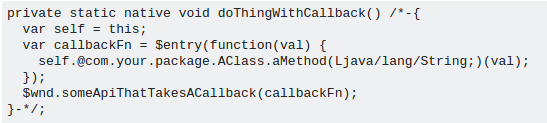
\includegraphics[width=1\linewidth]{jnsiexample}
\caption[Example of JSNI]{Example of JSNI. The keyword native modifies the method, so it can receive a comment beginning with /*- and ending with -*/, embedding Javascript code.}
\label{fig:jnsiexample}
\end{figure}

	In ZL, using the keyword \textbf{primitiva} and multi-line comment lets developers to write native Javascript code, as can be seen in \hyperref[fig:zlcode]{figure 1.2}.
	
	\begin{figure}
	\label{fig:zlcode}
	\centering
	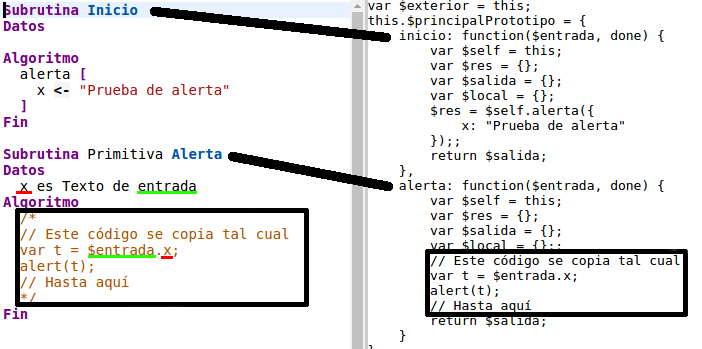
\includegraphics[width=1\linewidth]{zlyjs}
	\caption[Native JavaScript code written in ZL]{At left, ZL code. At right, JavaScript code. The keyword \textbf{primitiva} modifies the subroutine, so it must contain a multi line comment, embedding Javascript code.}
	\end{figure}
	
	There are plenty of functionality already written as native code using this technique. This functionality lets new students easily draw simple figures into a canvas, and also let them write text-based programs (with input and output of text). It is achieved by using HTML5 (Canvas, text input, ...) functionality embedded into ZL subroutines, and can be found at the directory \textbf{bibliotecasZL/*.zl} of the project.  

	As part of the programming environment, users can write ZL code directly in the web browser with the aid of an \textit{intelligent} editor. The intelligence provided to the editor relies on automatic suggestion of keywords and names, to aid students to auto-complete code without the need of memorizing full names. This is a key part of the project as ZL is a verbose language, and it may be harder to memorize than professional languages which are shorter to write.
	
	When a user writes code (of at least 3 letters) triggers the automatic suggestion which shows a list inside a popup with possible options \hyperref[fig:beforecompletion]{(Figure 1.3)}.
	
	
\begin{figure}
\centering
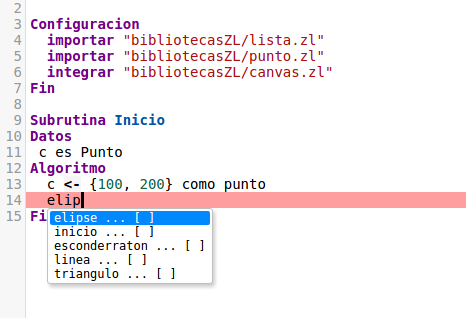
\includegraphics[width=0.7\linewidth]{beforecompletion}
\caption[Automatic suggestion]{Automatic suggestion. Writing partial names forces the editor to sort the possible options.}
\label{fig:beforecompletion}
\end{figure}

	Every time a programmer uses auto-completion, the editor fulfills a template for the structure selected by the user, so he/she does not have the need to remember the structure, arguments and names \hyperref[fig:aftercompletion]{(Figure 1.4)}.
	
\begin{figure}
\centering
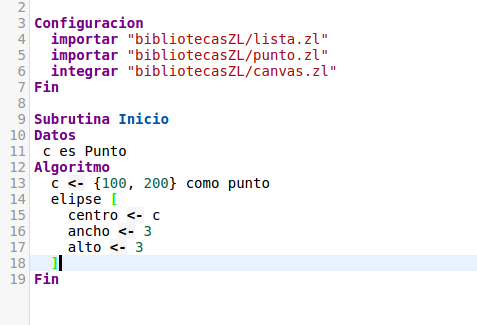
\includegraphics[width=0.7\linewidth]{aftercompletion}
\caption[Automatic completion]{Automatic completion. After selecting the `elipse' option, the editor fulfills all the arguments with a default value whenever possible.}
\label{fig:aftercompletion}
\end{figure}

	This part seemed really necessary because, as it was pointed out before, reading ZL may be easier, but writing may be (a lot) harder without any help. We see that remembering every argument of every subroutine is not an attractive feature for a language. In the case of new students, this will likely be a real problem. Memorizing structures (in ZL there are just two loop structures and three conditionals) composed by three or four keywords does not seem like a hard task. However, having to remember over fifty subroutines with two or more arguments (because return values in ZL are arguments too) will most likely be an issue. 
	
	Each time the code successfully compiles, one of the compilation stages generates a symbol table. This table is used to populate all the suggestions of the auto-completion. If a user writes a new subroutine, it is added into the table and therefore into the list of automatic suggestions.
	
	 For every possible option from the list, the editor calculates this distance between the suggestion and the user's input. This distance is Levensthein's distance\cite{levensthein}. After that, items with less distance appear first. That is the reason that makes `elip' show `elipse' before any other option in \hyperref[fig:beforecompletion]{figure 1.3}.
	
	The editor is also provided with syntax highlighting. If a line contains an error it is colored in pink (like `elip' line in \hyperref[fig:beforecompletion]{figure 1.3}). Every keyword is colored in dark pink, and every string in red. 
	
	If the code fails to be compiled because the user inputs wrong syntax, or it does not pass any semantic test, the user interface displays an error in common language to warn the user why the code is refused to be compiled. Errors are generated at the first three of the four compiling stages, as an exception (with helpful data to construct a message). The editor catches the thrown error, then calls a constructor using the thrown error, which generates an HTML code that is embedded into the user interface. 
	
	ZL code can be debugged by using breakpoints which are part of the code itself. Users can write `pausar' (pause) as a sentence inside an algorithm  which breaks the code in two parts: the code before the pause executes normally, then the code is stopped. A button in the user interface with a label `continuar' (continue) is shown. When pressed, this button will resume the execution of the code, running the second part (the one after the pause, \hyperref[fig:pausa]{figure 1.5}).  
	
\begin{figure}
\centering
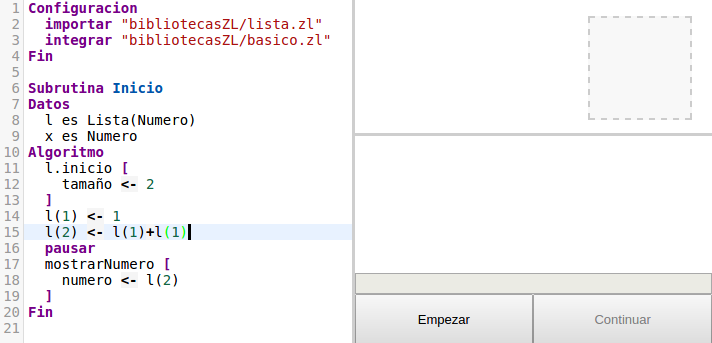
\includegraphics[width=0.48\linewidth]{pausa1}
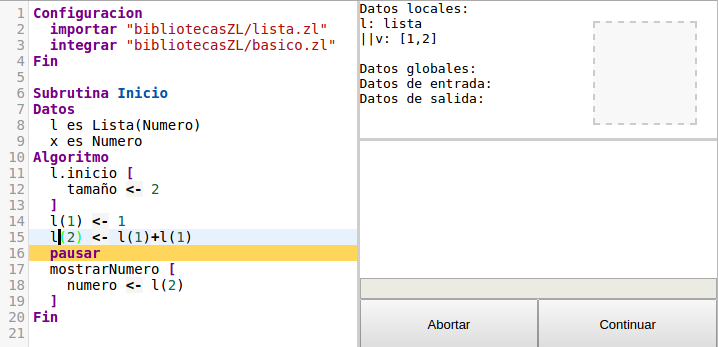
\includegraphics[width=0.48\linewidth]{pausa2}
\caption[Breakpoint: pause example.]{At the left, the code is written but not executed, and it contains a breakpoint at line sixteen. At the right the code is executed and paused at the breakpoint. The right top section of the interface shows debug information with the values of the variables at the moment of the pause. At the bottom right section we can see that the continue button is not enabled until the code is paused.}
\label{fig:pausa}
\end{figure}

	To end this abstract, it is rational to think that the aim of this tool is not giving users a professional language to produce programs. Having this tool may get new learners of computer programming less busy reading and writing code, and focusing more on how to produce and understand algorithms. We do not suggest advanced students to keep using ZL, but we suggest to move onto professional languages which have a bigger community, more efficiency, a greater number of tools to produce professional and maintainable code, and more testing of stability. 

	We hope that all these features will be helpful to new Spanish learners of computer programming, and also to teachers that will be able to create their own learning framework using ZL. It would be great to have the language tested by new users to measure the learning curve of this language inside this environment, to see what parts can be changed to get a better language in terms of learning success. 
	
	\chapter{Introducción}
	
	El objetivo fundamental de este trabajo es conseguir un entorno de desarrollo (o IDE) sencillo para aquellos que se inician en el mundo de la programación tengan una alternativa a las herramientas profesionales que si bien son muy útiles para los ingenieros informáticos también son más complejas de usar. Algunas de las técnicas usadas para simplificar este proceso se basan entre otras de abstraer al usuario del ciclo de compilación y ejecución, autocompletado de código y creación de un lenguaje de programación cercano al lenguaje natural español. 
	
	\vspace{10px}
	
	Si bien, el objetivo principal es que el proyecto se use por alumnos preuniversitarios (como Descubre, sistema del que se habla \hyperref[descubre]{más adelante}), cualquier persona que se inicie en la programación puede beneficiarse de este proyecto.
	
	\vspace{10px}
	
	Este trabajo se ha dividido en tres partes fundamentales: la creación de un lenguaje propio (se llamará ZL), un compilador para poder transformar tal lenguaje en otro que ya exista y se pueda, por tanto, acabar ejecutando; y un editor de texto que facilite la escritura de ese código en ZL.

	\vspace{10px}

	Algunos de los puntos que se han perseguido durante la creación de este trabajo son los siguientes:
	
	\begin{itemize}
		\item El lenguaje debe estar en la medida de lo posible en castellano. Es posible que iniciados que no conozcan inglés se beneficien de este punto.
		\item El lenguaje preferiblemente será tipado, con comprobación de tipos \cite{statictypecheck}\cite{typesafety} y sin operaciones de memoria \cite{memorysafety} (como los punteros de C o C++, que permiten el bypass de tipos). 
		\item El lenguaje tendrá tipos de datos con nombres comunes. Por ejemplo, se evitará el uso de Mapa y Vector, y se usarán nombres como Relación y Lista respectivamente. Se asume que una persona sin conocimientos matemáticos ni informáticos aceptaría nombres como Lista antes que Vector.
		\item No se debe asumir automáticamente conversiones de datos. Los alumnos deben ser conscientes de que los datos tienen un representación que se puede convertir, pero que el ordenador no tiene por qué asumir conversiones y hay que dar órdenes explícitas.
		\item Que no requiera instalador. Las instalaciones llevan tiempo y, aunque puedan ser instalaciones sencillas, requieren un esfuerzo.
		\item Si fuera posible, integrable con la herramienta Descubre, para aprovechar el sistema de usuarios y de compartir los ejemplos que ya tiene.
		\item Que sea flexible. Así los posibles docentes podrían añadir nuevo contenido a la herramienta.  
	\end{itemize} 
	
	\vspace{10px}
	
	Se espera que con estos puntos el proceso de desarrollo se simplifique hasta el punto de que se pueda atraer la atención de nuevos iniciados que, con otras herramientas quizá sientan más dificultades. 
	
	\section{Sugerencias para la lectura del documento}
	
	Todos los ficheros que se referencian en este documento deben poder encontrarse en \href{https://github.com/lilezek/zl}{https://github.com/lilezek/zl}. El código en el repositorio va cambiando con el tiempo, y es posible que algún ejemplo de la memoria se quede obsoleto tras un arreglo o una actualización del código. Sin embargo, hago referencia a este \textit{commit}: ec73f285a5a783ff0ec5142263f4e875b10f692b. Si hubiera grandes diferencias entre el documento y el proyecto, se recomienda clonar y analizar ese commit.
	
	El proyecto se puede probar en vivo en esta web: \href{https://lilezek.github.io/zl}{https://lilezek.github.io/zl}.
	
	\section{Ideas extraídas de los distintos proyectos}
	
	Durante el estado del arte se han localizado algunos puntos que considero importantes para el trabajo. Por ejemplo, uno de los proyectos (\textbf{Descubre}) define un lenguaje propio (\textbf{iJava}, un derivado imperativo de Java), al igual que este trabajo que define su propio lenguaje (ZL). Por otra parte, todos los proyectos estudiados coinciden en que se \textbf{desarrollan sobre web} y que \textbf{compilan de forma transparente}, y ofrecen un editor `inteligente' (con autocompletado, con coloreado de sintaxis...), objeto que se busca también en este trabajo. Se prefiere un lenguaje común antes que un lenguaje ingenieril, ya que es posible que sea más sencillo de entender para usuarios nuevos, a la hora de mostrar errores en la compilación (el proyecto Khan Academy \hyperref[app:d]{hace uso de esta técnica}).
	
	\chapter{Estado del arte}

	Se ha basado el estudio del arte en tres partes: la primera ha sido buscar proyectos enfocados al aprendizaje de la programación. Estos sitios aunque \hyperref[app:b]{estéticamente} parecen enfocados a personas jóvenes son muy útiles realmente para cualquiera que quisiera iniciarse (según afirman estos sitios).  
	
	Como todos los sistemas desarrollados son web, todos usan como tecnología HTML5 (Canvas para dibujar) y Javascript.

	La segunda parte ha sido enfocada en estudiar los diferentes analizadores gramaticales disponibles en Javascript. La creación de un lenguaje nuevo (ZL, del cual se habla más adelante) y su propio compilador (se descarta la opción de hacer un intérprete) impone la necesidad de usar alguna técnica de análisis del lenguaje. El compilador del lenguaje deberá compilar a Javascript para poder ser evaluado dentro del marco del explorador web.
	
	Por último, una vez que se tiene el lenguaje y el compilador, falta un editor para poder escribir el código que se va a compilar. En la práctica aquí no hago un estudio de distintas alternativas de editores de texto en HTML+Javascript porque previo al proyecto ya conozco una tecnología que ofrece todo lo necesario (en concreto, Codemirror de la cual se habla en su sección del estado del arte), y que además es la misma tecnología que usan proyectos de los cuales se estudia (Descubre, por ejemplo, integra su editor Codemirror para poder escribir código iJava).
	
	\section{Entornos de aprendizaje a la programación}
	
	En la introducción se habla de unos puntos que son objetivo de este trabajo. Parte de esos puntos son ya conocidos por mi propia experiencia de uso con estas herramientas, y otros puntos han surgido a la hora de estudiar los siguientes proyectos.
	
	\subsection{Descubre}
	
	\label{descubre}
	
	La herramienta Descubre, desarrollada por Juan Antonio Sánchez Laguna, Marcos Menárguez Tortosa, y Juan Antonio Martínez Navarro, reúne un editor de un lenguaje propio (\textbf{iJava}), un entorno con un editor de texto (\textbf{CodeMirror}, con coloreado de sintaxis entre otras ayudas a la escritura de código) y un entorno de ejecución que permite escribir \textbf{programas} de \textbf{entrada} (usando diálogos bloqueantes) y \textbf{salida} de texto (a un div HTML), o bien para \textbf{dibujar en un lienzo} de 320x320 (en HTML5 canvas).
	
	iJava es un lenguaje que retira de Java la orientación a objetos, convirtiéndolo en un lenguaje imperativo que respeta la sintaxis de Java. Parece 
	sensato pensar que este lenguaje es un buen puente entre los alumnos que se inician y quieran programar en Java en un futuro.
	
	Manual de iJava: \url{http://descubre.inf.um.es/aprende.php}
	
	El estilo de programación y las funcionalidades que ofrece están inspiradas en Processing, otro lenguaje y entorno de programación que prima la sencillez y se enfoca en el dibujado:
	
	Acceso: \href{http://processing.org/}{http://processing.org/}
	
	Otro punto destacable de esta herramienta es que \textbf{los usuarios pueden registrarse}, almacenar sus códigos para editarlos en un futuro y, si los usuarios marcan los \textbf{códigos} como \textbf{públicos}, \textbf{cualquiera puede clonar} el código y hacer una ramificación. 
	
	Usando esa parte de la herramienta, docentes como Ginés García Mateos han subido de forma pública a Descubre programas públicos (por ejemplo, una versión del Arkanoid) que alumnos pueden clonar y editar para sus propias versiones.
	
	\vspace{10px}
	
	Acceso: \url{http://descubre.inf.um.es}
	
	\subsection{Codecombat}
	
	CodeCombat es un proyecto de código abierto (en la teoría cualquiera podría sacar su propia plataforma, así como participar añadiendo nuevos problemas, clonando el proyecto en GitHub) para aprender a programar. Está compuesta de dos secciones, una multijugador donde enfrentas un algoritmo escrito en una especie de arena contra otros jugadores, y otra sección local donde resuelves problemas en un lenguaje a elegir para ir aprendiendo.
	
	\vspace{10px}
	
	El flujo de aprendizaje recomendado sería algo así: primero se resuelven los problemas que van creciendo en dificultad y, entonces, se participa en el modo multijugador. 
	
	\vspace{10px}
	
	Los problemas se basan en resolver unas especie de mazmorras donde el personaje principal tiene que conseguir unos objetivos, como defender unos puntos, eliminar a unos personajes controlados por inteligencia artificial, resolver un laberinto, etc... Las `arenas' multijugador sin embargo enfrentan a varias inteligencias artificiales de distintos jugadores entre sí para ver quien consigue el objetivo o la mayor puntuación.
	
	\vspace{10px}
	
	El entorno consta de varios lenguajes (Python, Javascript, Clojure, CoffeScript y Lua) donde adaptan cada problema al lenguaje. Por ejemplo, en problemas donde no se debe usar un bucle el propio entorno elimina (no compila, y muestra un error) el bucle del lenguaje para no poder usarlo. De esta forma, se `guía' a los aprendices sobre el uso de las estructuras del lenguaje.
	
	\vspace{10px}
	
	La complejidad de los problemas los han adaptado como si se tratase de un juego de rol. Cada vez que se resuelve un problema se consigue oro, con el que se pueden comprar objetos para equiparlos al personaje principal. Estos objetos añaden funcionalidad adicional al lenguaje. Por ejemplo, las botas básicas te permiten mover a las 4 direcciones (arriba, abajo, izquierda y derecha), pero otras botas más complejas te permiten mover al personaje directamente hacia un punto cualquiera del mapa a partir de sus coordenadas (además de las 4 direcciones), siguiendo el camino más corto (y ocultando el algoritmo que haya detrás de búsqueda del camino más corto).
	
	\vspace{10px}
	
	A todo esto hay que añadir que han hecho el esfuerzo de traducir la plataforma a varios idiomas. Si bien algunos problemas recientes no están traducidos, la gran mayoría del proyecto está en castellano (entre otros idiomas).
	
	\vspace{10px}
	
	Acceso: \url{http://codecombat.com}
	
	\subsection{Scratch}
	
	Scracth es un proyecto impulsado por el MIT para el desarrollo de pequeños proyectos con dibujos, animaciones y sonidos. Está enfocado para que niños programen y compartan contenido multimedia (historietas, animaciones e incluso juegos) con el resto del mundo. 
	
	Scratch carece de lenguaje escrito. Su editor ofrece un panel bidimensional en el que se pueden encajar unas piezas dentro de otras que equivalen a estructuras de control, sentencias de asignación, etc... Es un lenguaje dirigido por eventos donde un evento es una pieza a la que le siguen más piezas que equivalen a su funcionalidad. Los eventos son tales como \textbf{Al clickar}, \textbf{Al empezar}, \textbf{Al pulsar una tecla} (\hyperref[fig:scratch]{figura 3.1})
	
	
\begin{figure}
\centering
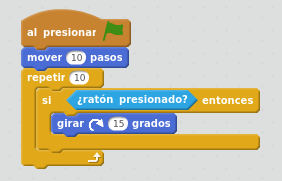
\includegraphics[width=0.7\linewidth]{scratch}
\caption[Ejemplo de Scratch.]{Ejemplo de Scratch, en castellano.}
\label{fig:scratch}
\end{figure}


	Las formas de las piezas y los colores representan distintos tipos de estructuras. Por ejemplo, las piezas con los lados en forma de pico (en la imagen, \textbf{¿ratón presionado?}) son elementos booleanos. Pueden entrar dentro de un \textit{if}. Como cada elemento tiene una forma dependiendo del tipo, los alumnos pueden asociar fácilmente qué estructuras `encajan' en otras. Formalmente hablando, el lenguaje no permite un error de compilación, ya que el editor solo permite añadir elementos allá donde sea válido.

	\vspace{10px}
	
	Scratch tiene un sistema de repositorios. Para hacerlo más amigable, cada proyecto se representa como un árbol, y cuando alguien lo clona aparece una nueva rama de tal árbol ( \hyperref[fig:scratch2]{figura 3.2} ).
		
\begin{figure}
\centering
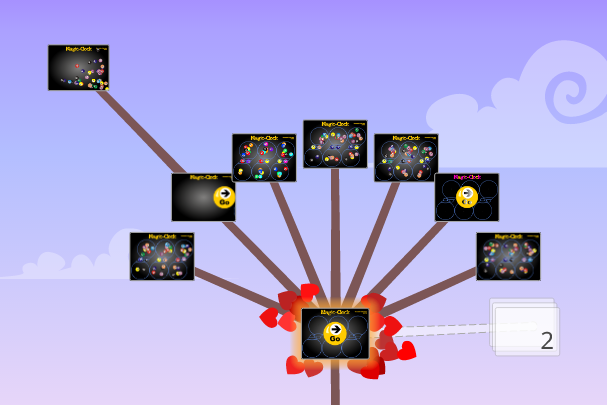
\includegraphics[width=0.7\linewidth]{scratch2}
\caption[Árbol de proyectos en Scratch.]{En el árbol se puede ver cada ramificación del proyecto principal, que está representado en el tronco.}
\label{fig:scratch2}
\end{figure}

	Este proyecto es mundialmente conocido, mantenido por un equipo dentro del MIT, y con una gran base de usuarios y proyectos distintos.
	
	Acceso: \url{https://scratch.mit.edu}
	
	\subsection{code.org}
	
	Si bien el entorno anterior (Scratch) ofrece un editor usando piezas para crear tus propios proyectos, code.org ofrece un editor similar. La diferencia está en que esta web ofrece problemas que hay que resolver, y no un entorno para crear tus propios programas.
	
	Funciona como el resto de los entornos dentro de la web con varios tipos niveles de problemas, donde hay un lienzo representando un problema. Los alumnos (recomendado de 4 a 18 años) resuelven unos problemas que crecen progresivamente en dificultad (\hyperref[fig:codeorg]{figura 3.3}). 
	
	\begin{figure}
	\centering
	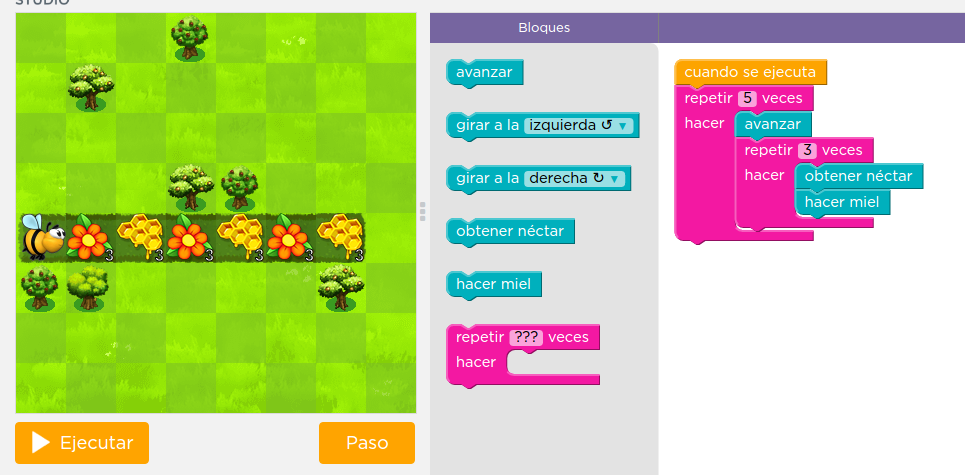
\includegraphics[width=0.7\linewidth]{codeorg}
	\caption[Resolviendo un problema en code.org]{A la izquierda, la representación visual y animada del problema. A la derecha, el editor con las opciones a elegir para resolver el problema.}
	\label{fig:codeorg}
	\end{figure}

	
	\vspace{10px}

	Los problemas son visualmente muy entretenidos (como los de codecombat), aunque más enfocados a alumnos más jóvenes (desde 4 años). Al igual que en Scratch, el entorno interpreta unos bloques paso a paso (para ver la animación del resultado) para comprobar si se ha resuelto o no el problema. 
	
	\vspace{10px}
	
	El entorno está traducido al castellano y dispone de vídeos introductorios con subtítulos al español.
	
	\vspace{10px}
	
	Acceso: \url{http://code.org}
	
	\subsection{Khan Academy - Aprendiendo a dibujar con Javascript}
	
	Khan Academy es una web que ofrece cursos interactivos sobre diversas ramas del conocimiento. A diferencia del resto de los trabajos estudiados, esta web es la única que no se dedica exclusivamente al aprendizaje de la informática y la programación.
	
	De entre todas existe una sección para aprender JavaScript. En esta sección se ofrecen distintos tutoriales en los que se va dibujando en un lienzo con unas llamadas sencillas (al estilo de Programming o Descubre). En los tutoriales se va progresando y se va enseñando como dibujar cosas más complejas, introduciendo los distintos elementos de JavaScript (bucles, asignaciones, funciones...) a través de una interfaz que reproduce unos pasos subtitulados al castellano y que interactúa con el editor de código.
		
	\vspace{10px}
	
	El editor permite la edición de casi cualquier valor usando un elemento gráfico (como por ejemplo, una paleta de colores para cambiar los colores de los elementos a dibujar). Además, el código se compila automáticamente y se pinta en el lienzo cada vez que el código cambia. El editor usa \hyperref[app:d]{lenguaje común} para describir entre otras cosas errores de compilación. A diferencia de los otros proyectos, el editor de código de Khan Academy es el más trabajado de todos, enfocándose principalmente en un editor con muchas funcionalidades y en tutoriales interactivos usando el editor.
	
	\vspace{10px}
	
	Acceso: 
	\href{https://es.khanacademy.org/computing/hour-of-code/hour-of-code-tutorial/p/intro-to-drawing}{Intro to Drawing}
	
	\subsection{Analizador ascendente: Jison}
	
	Jison es un proyecto escrito en Javascript que ofrece las herramientas similares a GNU Bison, un analizador de gramáticas libres de contexto de tipo LALR(1) \cite{bison}.
	
	El análisis se basa en dos fases: una primera fase rompe en tokens el texto (análisis léxico) y una segunda analiza los tokens y toma unas reglas u otras (análisis sintáctico).  
	
	Acceso:
	\href{https://github.com/zaach/jison}{Github de jison}	
	
	\subsection{Análisis descendente: pegjs}
	
	El analizador de gramáticas de expresiones\cite{peg} (en inglés Parsing Expression Grammar, o PEG) es un tipo de analizador que se define como más potente que cualquier LL(K) o LR(K)\cite{pegjs}. Tiene una herramienta online para probar el analizador que define un metalenguaje para definir las reglas de un lenguaje a analizar. Al igual que Jison está escrito en Javascript.
	
	Acceso a la prueba online:
	\href{http://pegjs.org/online}{http://pegjs.org/online}
	
	\subsection{Analizador descendente por prioridad de operadores}
	
	El analizador descendente (Top Down) por orden de prioridad de operadores (Operator Precedence) fue presentado por Vaughan Pratt en el año 73 \cite{acmtdop}. El analizador se basa en definir unos símbolos, unas expresiones y unos operadores (indicando su prioridad de forma numérica) con funciones recursivas que indican el comportamiento a la hora de ir avanzando recursivamente.
	
	Se puede encontrar más información sobre la teoría y una implementación del analizador en este sitio: 
	\href{http://javascript.crockford.com/tdop/tdop.html}{Texto de Douglas Crockford}
		
	\section{Editor de código y entorno de programación}
	
	El entorno está divido en 4 partes: editor de texto, lienzo de dibujo, apartado auxiliar para depuración, y apartado para entrada y salida de texto con botones de inicio y aborto de la ejecución.
	
	\subsection{Editor de texto HTML5 y Javascript}
	
	Lo primero que he encontrado ha sido el editor Codemirror. Es el mismo editor que usa el proyecto Descubre de la facultad. No me he dedicado en buscar otros editores porque este tiene
	todo lo que necesito para poder preparar el entorno, y además su API está muy bien documentada\cite{codemirrorapi}.
	
	Acceso:
	\href{http://codemirror.net/}{Página web oficial de codemirror.}
	
	\subsection{Coloreado de sintaxis}
	
	El propio editor de texto CodeMirror visto en el apartado anterior tiene elementos para configurar un autocompletado basado en tokens. 
	
	\vspace{10px}
	
	Cada token se clasifica en una clase u otra, y después cada clase tiene un estilo CSS asociado. De esta forma, con una buena clasificación y una hoja de estilos CSS se puede conseguir configurar este aspecto del editor.
	
	\subsection{Autocompletado}
	
	Existe un plugin para facilitar el autocompletado de código para CodeMirror, aunque solo ofrece un menú contextual al escribir texto. 
	
	\vspace{10px}
	
	A este plugin habría que añadirle la funcionalidad sobre qué elementos deben aparecer en el menú contextual, así como en qué orden y qué acción realizaría cada elección.
	
	\subsubsection{Elementos para la lista de autocompletado}
	
	Editores como Code::Blocks (para C++) y Eclipse (para Java) permiten autocompletar estructuras (sintácticas del lenguaje) así como nombres (de funciones, de métodos, de clases, de variables...).
	
	\vspace{10px}
	
	En el menú contextual también se muestra información adicional sobre los métodos en Java, si estos han sido previamente comentados usando algún estándar como Javadoc\cite{javadoc}.
	
	\vspace{10px}
	
	Las entradas de los menús contextuales a la hora de sugerir opciones para autocompletar varía dependiendo de la posición donde se está escribiendo el código, así como del código incluido previamente. En otras palabras, el autocompletado se puede hacer sensible al contexto y entonces dependería del código escrito anteriormente, ofreciendo mejores resultados.
	
	\subsection{Compilado transparente - Autocompilado}
	
	Todos los entornos de aprendizaje vistos con anterioridad tienen un botón para iniciar la ejecución, pero el compilado es transparente. Sin embargo, los usuarios reciben un mensaje de error cuando cometen un error al escribir código, lo que da a pensar que el código se está compilando (o al menos, analizando) de forma periódica, automática y transparente mientras el usuario escribe. 
	
	\vspace{10px}
	
	Todo apunta a que cuando el usuario deja de teclear durante un corto periodo de tiempo, se inicia la compilación. Esta compilación se almacena para su posterior uso, ya sea para mostrar un mensaje de error o para permitir el inicio de la ejecución, al pulsar un botón de inicio.
	
	\chapter{Análisis de objetivos y metodología}
	
	%TODO: Edu: ¿Capítulo vacío?
	
	\section{Objetivos para un nuevo entorno de aprendizaje de programación}
	
	Los objetivos principales han sido crear un lenguaje con palabras cercanas al lenguaje común español, un editor de texto inteligente y un compilador de dicho lenguaje, buscando en la medida de lo posible la facilidad y la utilidad. 
	
	\vspace{10px}
	
	El primer objetivo pasa por definir el lenguaje. Este objetivo es básicamente encontrar una forma de definir el lenguaje, en el cual me acabé decantando por la forma de Backus-Naur\cite{bnf} con alguna modificación, aunque también estudié la posibilidad de usar DCG\cite{dcg} pero la descarté por parecer más compleja de entender. 
	
	\vspace{10px}

	El segundo objetivo es escribir el compilador, pero para ello es necesario un entorno para poder probar el el propio compilador, así que como objetivo intermedio se hizo el editor. Se escogió Codemirror porque es sencillo, tiene buena documentación, ofrece un plugin para colorear texto\cite{codemirrorsyntaxhighlight} y otro para autocompletar\cite{codemirrorautocomplete}. 
	
	\vspace{10px}
	
	Una vez definido lenguaje y  con un editor en el entorno, falta el último objetivo, que es el compilador de dicho lenguaje. Tal compilador debe ser capaz de compilar el lenguaje definido como primer objetivo, el cual tiene ambigüedades porque usa lenguaje cercano al lenguaje natural.
	
	\section{Definición del lenguaje ZL}
	
	A la hora de definir el lenguaje ZL el esfuerzo se ha enfocado en que fuese cercano al lenguaje natural, y que estuviese en español\cite{mundoingles}. Si bien la definición del lenguaje se podría someter a pruebas (como encuestas) para comprobar su eficacia y pulir los defectos y deficiencias que pudiera tener, se ha basado principalmente en mi experiencia como programador. 
	
	\vspace{10px}
	
	El léxico se ha escogido por su cercanía al lenguaje natural, y no en base a su `practicidad'. Si asumimos que es práctico usar palabras cortas y estructuras sencillas como podría ser bucle `while' de C (y de Java, C\#...) se ha preferido usar estructuras más cercanas al lenguaje humano: `mientras \textit{se de una condición} hacer \textit{un conjunto de pasos} fin', aunque sean más largas de escribir y más complejas de analizar.
	
	\vspace{10px}
	
	Por otro lado, los nombres escogidos se intentan alejar del lenguaje técnico informático (salvo ciertas palabras clave, como Subrutina y Algoritmo). Se ha preferido nombres como `Lista' y `Relacion' frente a `Vector' y `Mapa'. Se ha escogido el nombre `Dato' frente a `Variable'. Se usan palabras para abrir y cerrar bloques como `Hacer' y `Fin' en vez de las llaves \{\} que se usan en C o en Java. 
	
	\vspace{10px}
	
	\subsection{Notación BNF ampliada}
	
	La notación BNF que utilizo para dar una definición formal al lenguaje es una notación BNF a la cual he añadido paréntesis para agrupar, y los operadores *, + y ? como operadores de repetición. Funcionan como en las expresiones regulares: * para indicar cero o más veces, + para indicar uno o más veces, y ? para indicar cero o una veces. También utilizo los corchetes [
	] para agrupar un conjunto opcional (cero o una veces), equivalente a usar paréntesis y el símbolo ?.
	
	\vspace{10px}
	
	Los siguientes ejemplos son equivalentes en BNF:
	
	\begin{BVerbatim}
BNF extendido:
a ::= b c?
x ::= (y z)*
j ::= k (l m)+
	
BNF:
a ::= b
  | b c

j_plus ::= l m
       | j_plus l m	

j ::= k j_plus

x ::= 
  | y z x
	\end{BVerbatim}
	
	Por último, utilizo los puntos y comas para indicar comentario.
	
	\subsection{Descripción del lenguaje}
	
	En el \hyperref[app:a]{apéndice A} (o el documento sintaxis.txt) se puede encontrar la definición formal en BNF extendido del lenguaje. En esta sección se va a explicar con ejemplos qué estructuras sintácticas se buscan para el lenguaje, siempre siguiendo como guía el documento del \hyperref[app:a]{apéndice A}. En el documento se usa reiteradas veces la estructura \_ que indica un número arbitrario de espacios, opcionales donde no cause ambigüedad. 
	
	\vspace{10px}
	
	Los comentarios no se incluyen en la definición formal del lenguaje, aunque se deberán ignorar todos los segmentos de código que contengan comentarios con el estilo de C/C++/Java. La doble barra // hasta final de línea, o los comentarios multilínea /* y */.
	
	\vspace{10px}
	
	El lenguaje es totalmente insensible a mayúsculas y minúsculas salvo para los literales de tipo texto. Es decir, cualquier nombre o palabra reservada se acepta en cualquier combinación de mayúsculas y minúsculas y no altera el comportamiento. Sin embargo, los literales de texto si difieren en mayúsculas o minúsculas, y pueden alterar el comportamiento.
	
	\vspace{10px}
	
	La primera parte del apéndice define formalmente que un número puede ser un entero o decimal, qué es un \textbf{módulo}, qué es una \textbf{configuración} y qué es una \textbf{subrutina}. Se obvia la definición de número pues es muy sencilla (define las constantes numéricas para el lenguaje), y nos centramos en la definición de módulo: la estructura sintáctica más grande. Cualquier código que sea compilable ZL tiene que seguir la definición de módulo. Así pues, un módulo es la unidad mínima compilable.   
	
	\vspace{10px}
	
	Un \textbf{módulo} se compone de una \textbf{configuración} (opcional) y de un número arbitrario de \textbf{subrutinas}. Con esta definición, un módulo podría ser un documento en blanco, sin configuración y con cero subrutinas. Las únicas restricciones que impone la estructura sintáctica de módulo son: la configuración solo puede aparecer \textbf{una vez al principio del documento}, y después pueden venir un número arbitrario de subrutinas. 
	
	\vspace{10px}
	
	La estructura \textbf{configuraciones} recoge cero o más estructuras de tipo \textbf{configuración}. Agrupa configuraciones donde se asignan constantes numéricas, constantes de texto, o se importan/integran otros módulos:
	
	\vspace{10px}
	
\begin{BVerbatim}
Configuracion
	precision <- 4
	nombre <- "Modulo"
	importar "Otromódulo.zl"
Fin
\end{BVerbatim}
	
	La segunda estructura que se puede encontrar en un \textbf{módulo} es la \textbf{subrutina}. La \textbf{subrutina} es la unidad máxima de ejecución. Contiene la definición de un léxico, y la definición de un algoritmo usando tal léxico. Por lo tanto, se separa en dos partes (cabecera y cuerpo):
	
\begin{BVerbatim}
Subrutina Hipotenusa
Datos
	CatetoA es Numero de Entrada
	CatetoB es Numero de Entrada
	Hipotenusa es Numero de Salida
Algoritmo
	raizCuadrada [
		numero <- CatetoA*CatetoA + CatetoB*CatetoB
		resultado -> Hipotenusa
	]
Fin
\end{BVerbatim}

	\vspace{10px}
	
	Primero se ha de escribir la \textbf{cabecera} de la subrutina. La cabecera contiene el nombre de la subrutina, que se usará para ser almacenada en la taba de símbolos por su nombre, y más tarde ser utilizada por otras subrutinas. Opcionalmente contiene también unos modificadores de subrutina, que son unas palabras clave que alteran el comportamiento del análisis y la semántica de la subrutina, de lo cuál se hablará más adelante.
	
	\vspace{10px}
	
	En el \textbf{cuerpo} de la subrutina obligatoriamente aparecen los \textbf{datos} (definición del léxico) y el \textbf{algoritmo} (sobre el léxico definido) en ese orden. En los datos se indica la definición de cada uno de los elementos del léxico, con un nombre, un tipo de datos, y un modificador (opcional) de ámbito (local, global, o de entrada o salida). Los modificadores de ámbito son los que dicen cuales van a ser los datos de salida (datos devueltos por la subrutina), los datos de entrada (argumentos de la subrutina), datos locales y datos globales (datos compartidos entre subrutinas). En el algoritmo se reúnen \textbf{sentencias}, que son los pasos a realizar sobre los datos definidos. Las operaciones (lecturas o escrituras) están restringidas si los datos son de entrada o de salida.   
	
	\vspace{10px}
	
	Una \textbf{sentencia} es la unidad mínima de ejecución. Hay distintos tipos de sentencias y algunas pueden contener más sentencias en su definición, como son las estructuras \textbf{bucles} \textbf{mientras} y \textbf{repetir}, o la estructura \textbf{condicional} \textbf{\textit{sicondicional}}. 
	
	\vspace{10px}
	
	La sentencia más simple es la sentencia de tipo \textbf{asignación}:
	
	\vspace{10px}
	
\begin{BVerbatim}
dospi <- 3.1415*2
array(1) <- 0
\end{BVerbatim}
	
	\vspace{10px}
	
	La \textbf{asignación} se define como un nombre ($dospi$) o un lvalor\footnote{Un lvalor o un valor izquierdo es la estructura sintáctica del lenguaje que se acepta en el lado izquierdo de una asignación. Pueden ser nombres o nombres seguidos de un acceso, como en el segundo ejemplo.}, seguido de una flecha que apunta hacia la izquierda (para que se intuya que la información `fluye' de derecha a izquierda) y finalmente seguido de una expresión. Las expresiones son similares a las expresiones que se pueden encontrar en Java o en C, sustituyendo ciertos operadores por otros operadores:
	
	\vspace{10px}
	
\begin{BVerbatim}
&& => y 
|| => o
! => no 
!= => <>
\end{BVerbatim} 

	\vspace{10px} 
	
	Por otra parte, además de los bucles y las asignaciones, están las sentencias \textbf{llamadas} que hacen uso de otras subrutinas. En ZL, la asociación de los argumentos que se pasan a las subrutinas se hace por nombre, y no por orden (como Java o C). Es decir, hay que conocer el nombre de los datos de entrada y de salida, y su orden no tiene importancia:
	
	\vspace{10px}
	
\begin{BVerbatim}
elipse [
	ancho <- 100
	alto <- 150
	centro <- {0,0} como punto
]
\end{BVerbatim}	

	\vspace{10px}

	Por último, existe una sentencia \textbf{pausar} que no realiza ningún cambio en la ejecución. Es un equivalente a un punto de pausa. Ofrece al lenguaje la posibilidad de parar la ejecución, de forma sencilla con una única sentencia, para analizar y depurar con detalle la ejecución del programa.
	
	\vspace{10px}
	
	Sobre todo este resumen de la descripción del lenguaje hay que añadir lo siguiente para que sea completa la descripción:
	
		
	\noindent Existe un `operador' (que no opera dos valores, sino un valor y un tipo) de conversión de un tipo a otro tipo. Este operador es el operador `como' y es el primero en el orden de precedencia. Un ejemplo de uso podría ser el siguiente:
	
	\begin{BVerbatim}
	mensaje <- "cuatro y dos hacen " + 42 como texto + "."
	\end{BVerbatim} 
	
	Además, el orden de los operadores se define usando varios `niveles' de expresiones y operadores.
	Por último, en ZL existe la genericidad (tipos que operan con tipos abstractos) sobre ciertos tipos, como lista. Un ejemplo de definición de lista sería el siguiente:
	
\begin{BVerbatim}
	matriz es Lista(Lista(Numero))
\end{BVerbatim}

	Y sería equivalente a la declaración en Java:
	
	\begin{BVerbatim}
	Vector<Vector<Dobule>> Matriz...
	\end{BVerbatim}
	

	\section{Desarrollo de un entorno de programación}
	
	Al igual que Descubre o Codecombat, el principal objetivo del trabajo es crear un entorno para facilitar la programación. Este sistema debe estar compuesto de al menos un editor de texto, el compilador del lenguaje diseñado y las herramientas de entrada y salida (barras de texto para escribir, lienzos para dibujar, eventos de teclado...). Recomendablemente el entorno debe tener información sobre depuración (errores al escribir el código, información de depuración al pausar el código, etc...) como tienen también otros entornos (Descubre o Codecombat, por ejemplo).
	
	\subsection{Editor de texto inteligente}
	
	Cuando se habla de editor de texto inteligente se habla de ciertas características que tienen ciertos editores como Eclipse o Code::Blocks entre las que se encuentran el coloreado, la \textit{autotabulación}, el autocompletado... 
	
	\vspace{10px}
	
	El objetivo de esta parte del trabajo es intentar imitar esas características sobre ZL. Por una parte, habrá que identificar cuales son los distintos tokens del lenguaje (números, palabras clave, cadenas literales de texto, comentarios...) para hacer una clasificación y un coloreado a cada clase. Es sabido que el coloreado de sintaxis es una parte fundamental a la hora de reducir el tiempo de lectura del código a analizar para nuevos alumnos, como indica el trabajo de Advair Sarkar\cite{syntaxhighlight}.
	
	\vspace{10px}
	
	Por otra parte también se plantea el objetivo del autocompletado. Según los laboratorios de investigación de Microsoft, el autocompletado con tolerancia a errores es útil para reducir los tiempos de escritura\cite{microsoftresearchautocomplete}. Por la naturaleza verbosa de ZL (donde las llamadas usan argumentos con asociación por nombre y no por orden), se encuentra de especial utilidad a la hora de escribir código las opciones de autocompletado, para no tener que memorizar nombres de subrutinas además de nombres de los argumentos en las subrutinas. 

	\vspace{10px}

	El tipo de autocompletado, además de tolerante a errores, se busca que tenga también conocimiento del contexto. Por ejemplo, reduciendo el número de palabras que autocompletar a solo aquellas que puedan encajar sin causar un error de compilación, o autocompletando las llamadas con unos valores por defecto. Se puede ver en la \hyperref[fig:completion]{figura 4.1} como se autocompletaría en base al contexto.
	
\begin{figure}
\centering
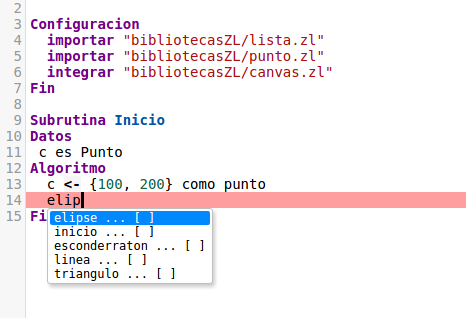
\includegraphics[width=0.4\linewidth]{beforecompletion}
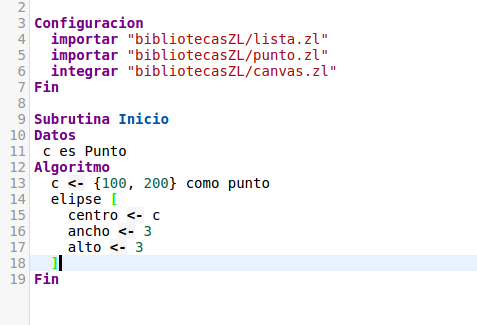
\includegraphics[width=0.4\linewidth]{aftercompletion}
\caption[Ejemplo de autocompletado.]{A la izquierda, el menú contextual que aparece cuando un usuario escribe `elip'. Para ello antes se ha debido importar \textbf{canvas.zl}, pues sino la subrutina elipse no formaría parte del entorno en ese contexto. A la derecha, el código que aparece autocompletado inmediantamente después de haber pulsado \textit{enter}.}
\label{fig:completion}
\end{figure}
	
	El funcionamiento y la implementación del autocompletado se ve más adelante en la sección \textbf{Editor inteligente - Autocompletado}.
	
	\subsection{Compilador de ZL a Javascript}
	
	Imitando a todas las plataformas estudiadas en el estado del arte, se establece como objetivo fundamental que el compilador de ZL se pueda integrar bajo un entorno web. Por ende, tiene sentido que el compilador genere código Javascript, y esté además escrito en Javascript. 
	
	\vspace{10px}
	
	El compilador tiene que ser capaz de traducir código escrito en ZL, y generar un código (y solo uno) Javascript que al ser evaluado en el explorador, genere la ejecución semánticamente equivalente. 

	\vspace{10px}
	
	Para el entorno de ejecución se establecerá un sistema dirigido por eventos. A la hora de evaluar el código, se pasarán una lista de eventos para que el código generado a partir del ZL tenga acceso de entrada y salida \hyperref[fig:diagramaeventos]{(figura 4.2)}:

\begin{figure}
\centering
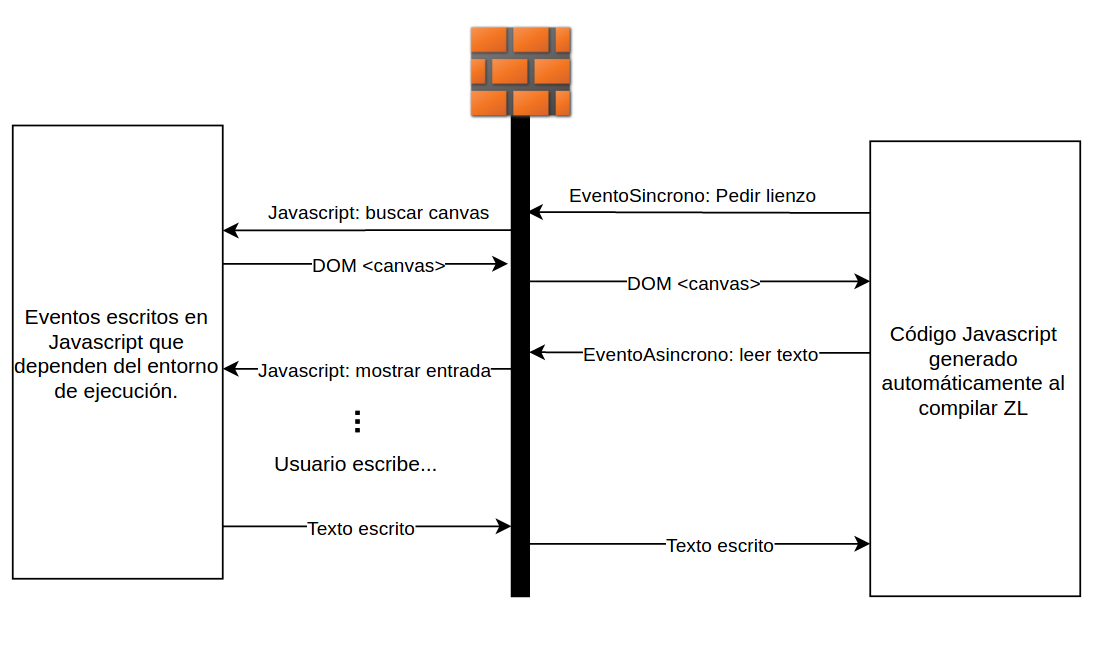
\includegraphics[width=1\linewidth]{diagramaeventos}
\caption[Diagrama de ejemplo de intercambios usando eventos.]{Ejemplo de llamadas a los eventos. El compilador generará código que llame a eventos cuando sea necesario, para obtener información del exterior (entrada) o para mostrarla (salida).}
\label{fig:diagramaeventos}
\end{figure}

	\chapter{Diseño y resolución del trabajo realizado}
	
	\section{Compilador de ZL}
	
	Todo analizador se puede ver como una máquina de estados que, por cada paso que se da, cambia su estado y consume una parte de la entrada a analizar. La complejidad de la máquina de estados puede variar, permitiendo análisis más o menos complejos. Para ZL, el compilador define tres fases de análisis más una cuarta fase de generación de código (\hyperref[fig:fasesanalisis]{figura 5.1}).
		
		
\begin{figure}
\centering
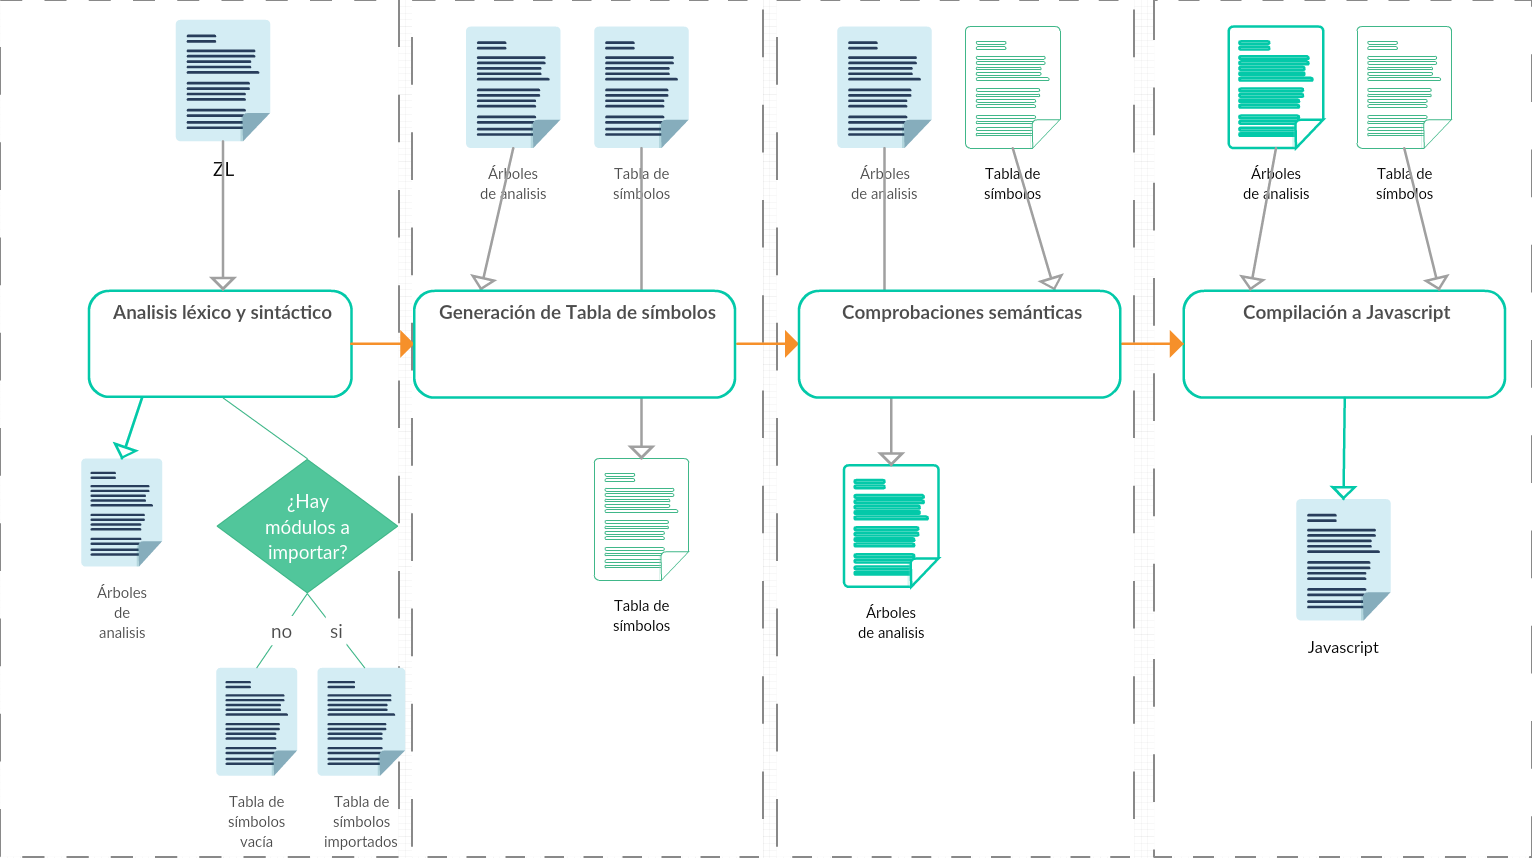
\includegraphics[width=1\linewidth]{fasesanalisis}
\caption[Fases de compilación.]{De izquierda a derecha, las 4 fases de la compilación en el orden en el que se ejecutan. }
\label{fig:fasesanalisis}
\end{figure}

	
	\vspace{10px}
	
	Durante estas fases se generan estructuras de datos cada vez más complejas, que permiten una conversión a Javascript. Salvo durante la primera fase, todas las fases trabajan con estructuras en forma de árbol (la tabla de símbolos y un árbol de análisis). Durante el análisis inicial (sintáctico y semántico) el analizador debe generar el primer árbol a partir de una cadena de símbolos, que son el texto del código a compilar. La implementación de esta parte pasa por usar una máquina de estados en el que se mantiene \textbf{una pila de colas de elementos} a avanzar, así como \textbf{la posición del siguiente carácter a leer} en el próximo avance. De esto se habla en más detalle en la sección `Pila de colas auxiliares para el análisis descendente recursivo'. 
	
	\vspace{10px}
	
	Las siguientes fases trabajan con árboles. De la primera fase se obtiene un árbol que representa las estructuras sintácticas, que en la segunda fase se usa para extraer nombres (de subrutinas, de datos...) y rellenar una tabla de símbolos\footnote{Tabla que relaciona nombres de subrutinas, nombres de variables, etc... con sus estructuras.}. La tabla de símbolos se rellena realizando una normalización y adicionalmente, durante este proceso se realizan ciertas comprobaciones semánticas (nombres no repetidos, tipos de datos existentes...), lanzando una excepción en caso de conflicto. De este análisis se habla con más detalle en la sección `Análisis sintáctico', y la definición de los elementos que componen la tabla están en `Tabla de símbolos'.
	
	\vspace{10px}
	
	En la tercera fase se realizan comprobaciones semánticas para cada una de las sentencias dentro de las subrutinas. Se analiza cada sentencia en busca de código ilegal: nombres que se usan pero no existen, operaciones entre dos tipos de datos no válidos, etc... con el objetivo de lanzar una excepción y detener el proceso de compilación en caso de encontrar alguna. Durante esta fase se altera el árbol inicial generado en la primera fase, añadiendo para cada expresión qué tipo de datos tiene como resultado. Por ejemplo, el árbol que represente $2 * 7$ tendrá en su información que el resultado es de tipo `numero'.  Se profundiza en esta fase en la sección `Análisis semántico'.
	
	\vspace{10px}
	
	En la cuarta y última fase se genera el código Javascript. Para ello se usan el árbol generado en las fases anteriores así como la tabla de símbolos. Se recorre el árbol de forma recursiva obteniendo las subrutinas del módulo, generando una función Javascript por cada subrutina. Los detalles de la generación de código Javascript se puede ver en los apartados `Código nativo, implementación de las subrutinas nativas' y `Código asíncrono convertido en código bloqueante'.
	
	\subsection{Justificación de la elección de análisis descendente recursivo}
	
	%TODO: Revisar léxico reducción derivación
	
	Después de analizar las distintas alternativas de analizadores para Javascript se optó por usar PEG.js. Sin embargo, se detectó una ambigüedad en la cual hay que avanzar hasta 3 tokens para determinar la regla de reducción correcta. Después de varios intentos con PEG.js por analizar la ambigüedad se descartó la herramienta. 
	
	\vspace{10px}
	
	Como la otra herramienta (Jison) ofrece un análisis LALR(1) de un solo token de anticipación se acabó optando por una solución personalizada: un analizador descendente (se inicia el análisis buscando la estructura más grande) recursivo (los no terminales, a los que llamo reglas, tienen asociada una función). 
	
	\vspace{10px}
	
	De las posibles alternativas se ha escogido un análisis descendente por que es más intuitivo (y más fácil de depurar), y un análisis recursivo para poder tener el control de cómo se debe avanzar (o incluso retroceder, en caso de ambigüedad) cada regla. 
	
	\vspace{10px}
	
	A diferencia de, por ejemplo Jison, cada regla tiene una función asociada para calcular el resultado de la derivación, pero y he aquí la diferencia, cada función asociada debe indicar también como se ha de avanzar.
	
	\vspace{10px}
	
	Se ha visto necesaria esta forma de hacer las reglas de reducción para obtener control total tanto de los errores al no poder avanzar como para solucionar las ambigüedades. 
	
	\subsection{Pila de colas auxiliares para el análisis descendente recursivo}
	
	Para los mecanismos de avance y retroceso se han diseñado unas funcionalidades que facilitan al desarrollador (en vías futuras podrían ser otros desarrolladores ajenos a este trabajo) a escribir las reglas de avance. 
	
	\vspace{10px}
	
	Todas estas funcionalidades hacen uso de una pila de colas de elementos (terminales o no terminales). En un momento dado, el analizador está en un estado (que es una cola), y cuando se va a avanzar, se desencola un elemento. Antes de avanzar, se apila ese estado, (después de haber desencolado el elemento). Entonces se inicia el avance (se llama a la función asociada a la regla). Cuando se acaba el avance, se desapila el estado, para recuperar el estado y continuar desencolando. Las colas contienen elementos que pueden ser reglas (no terminales), o tokens o símbolos (terminales).
	
	\vspace{10px}
	
	\textbf{Nota al lector}: se recomienda que esta sección, que contiene las definiciones de los métodos del analizador, se lea acompañando a las dos siguientes secciones: `Tratamiento de la recursividad izquierda' y `de la ambigüedad', donde se hacen uso de estos métodos con ejemplos. 
	
	\vspace{10px}
	
	Inicialmente, \textbf{la pila está vacía}. El cursor que apunta al texto a analizar está en 0 (posición inicial). A partir de ese estado, las funcionalidades que hacen uso de la pila de colas son las siguientes:
	
	\vspace{10px}
	\noindent
	\textbf{avanzarUno}: \textbf{parte principal del analizador}. Desencola un elemento de la cola actual. Después, apila la cola actual. Entonces, si el elemento es un no terminal, se llama a la función asociada, con una nueva cola vacía. En caso de ser un terminal, se intenta avanzar usando las expresiones regulares asociadas al terminal, avanzando el cursor tantos caracteres como se han leído, y saltando espacios y comentarios. Si no se pudo avanzar (la expresión regular no hace match) se propaga una excepción. Las funciones asociadas a reglas pueden lanzar excepciones también, para que los desarrolladores puedan propagar errores que no sean puramente léxicos.
	
	\vspace{10px}
	\noindent
	\textbf{avanzar}: si se llama con un argumento, vacía la cola actual e introduce en la cola el argumento, que puede ser un token, un símbolo o una regla. Después, (independientemente de si se llama con algún argumento o no) realiza `avanzarUno' a todos los elementos de la cola.  \textbf{avanzar('miregla')} equivale a \textbf{acumular('miregla')} y después \textbf{avanzar()}.
	
	\vspace{10px}
	\noindent
	\textbf{retroceder}: retrocede uno o varios tokens ya avanzados, símbolos, reglas. Si no se ha avanzado nada el comportamiento es no definido. Es útil para retroceder tokens avanzados en casos de ambigüedad, después de comprobar si el 2º o el 3er token no es el esperado. 
	
	\vspace{10px}
	\noindent
	\textbf{acumular}: encola un token, un símbolo o una regla. Útil para preparar la cola para usarla con otros métodos de avance.
	
	\vspace{10px}
	\noindent
	\textbf{intentar}: recibe un array bidimensional de opciones. Cada array dentro del array representa una cola en orden de izquierda a derecha. Esta utilidad intenta avanzar las distintas colas hasta que consigue avanzar una cola por completo. Si no se consigue avanzar ninguna se propaga una excepción. Si se consigue avanzar una cola parcialmente pero se encuentra con un elemento que no se puede avanzar se lanza una excepción. Por lo tanto, las colas deben fallar en el primer elemento, o acertar en todos para que el intento sea efectivo.
	
	\vspace{10px}
	\noindent
	\textbf{intento}: acumula en la cola un array bidimensional como el descrito en el método anterior. El método anterior \textbf{intentar} equivale a primero hacer un \textbf{intento} para acumular en la cola seguido de \textbf{avanzar} para avanzar la cola.
	
	\vspace{10px}
	\noindent
	\textbf{avanzarVarios}: avanza la cola tantas veces como se pueda. Antes de empezar a avanzar la cola se mantiene una copia (profunda) de la cola. Si se consigue avanzar la cola, se vuelve a intentar avanzar la copia, tantas veces como se pueda antes de que se capture una excepción.   
	
	\vspace{10px}
	\noindent
	\textbf{avanzarVariosObligatorio}: al igual que \textbf{avanzarVarios} avanza la cola tantas veces como se pueda, pero si no se puede avanzar al menos una vez entonces se propaga la excepción capturada.
	
	\vspace{10px}
	\noindent
	\textbf{arbol}: después de avanzar reglas, tokens o símbolos, se generan ramas, una por cada vez que se llame a \textbf{avanzar}, \textbf{avanzarVarios}, \textbf{avanzarVariosObligatorio} o \textbf{intentar}. Si se avanzan n veces, se generan n ramas, siendo la primera la rama 0. \textbf{arbol(2)} accede a la rama generada por el 3er avance. Si se llama sin argumento se obtiene el árbol de la regla actual, es decir, el nodo padre de todas estas ramas. El árbol para cada regla inicia vacío.
	
	\vspace{10px}
	\noindent
	\textbf{registrarResultado}: asocia al nodo del árbol de la regla actual un resultado, que se utilizará para obtener información tratada del análisis. Cuando se avanza un terminal el resultado equivale al texto completo que hizo \textit{match} a la expresión regular. Sin embargo, las reglas no terminales deben registrar de forma explícita su resultado. 
	
	\vspace{10px}
	\noindent
	\textbf{resultado}: se utiliza para obtener los resultados de los avances, registrados por el método \textbf{registrarResultado} o por el \textit{matching} de expresiones regulares. Existe un paralelismo entre el método \textbf{arbol} y el método \textbf{resultado}: si \textbf{arbol(2)} devuelve el árbol de análisis del tercer avance, \textbf{resultado(2)} devuelve el resultado previamente registrado del tercer avance.

	\vspace{10px}
	
	Cuando se avanza un \textbf{intento}, el resultado de ese avance es un entero que indica el índice del intento que salió bien. Es decir, si en un intento se pasan 3 colas, y se puede avanzar la última, el resultado de ese avance será el número 2. 
	
	\vspace{10px}
	
	Cuando se avanza con \textbf{avanzarVarios} o \textbf{avanzarVariosObligatorios} el resultado es un array con cada uno de los resultados individuales. Si se avanza 7 veces la misma cola, se obtiene un array de longitud 7 cuyos elementos son el resultado de cada uno de los avances individuales. 
	

	\subsection{Tratamiento de la recursividad izquierda}
	
	Por ser este analizador recursivo y descendente ninguna regla puede contener recursividad por la izquierda. La recursividad es el problema que desemboca en una recursión infinita cuándo una regla se contiene a sí misma en su definición como el primer elemento a reducir (y por ello está en la izquierda). Si se intentase avanzar tal regla, para poder avanzar debería reducirse a si misma de nuevo, cayendo en un bucle sin fin.
	
	Supongamos como regla recursiva por la izquierda la concatenación de nombres separados por punto que se pueden realizar en lenguajes orientados a objetos como Java (System.out.println por ejemplo), y para hacerlo un poco más complejo se permiten números también. Si se quisiera analizar el nombre con la siguiente regla:
	
	
\begin{BVerbatim}
; Ejemplo de texto válido 
System.14.out.println

; Expresiónes regulares para terminales
nombreSimple ::= <(\w+)>
numero ::= <(\d+)>

; Regla para el análisis
nombre ::= <nombre> . <nombreSimple> ; Recursivo izquierda
	| <nombre> . <numero> ; Recursivo izquierda
	| <nombreSimple> ; No recursivo
	| <numero> ; No recursivo
\end{BVerbatim}	

	Para que la regla se pueda avanzar correctamente, tiene que existir al menos una alternativa en la regla que no sea recursiva por la izquierda. Si todas fueran recursivas por la izquierda, se debe factorizar por la izquierda primero para obtener reglas equivalentes con al menos una sin recursividad\cite{conflictoll3}. Como en este caso ya hay una alternativa no recursiva, se puede escribir el código que trata con la recursividad:
	
\begin{BVerbatim}
{
  // Primero, se debe avanzar las opciones no recursivas.
  this
    .intentar([
      ["nombreSimple"],
      ["numero"]]);
  // Después se avanza tantas veces como se 
  // pueda el resto de las opciones recursivas,
  // pero sin incluir en el 
  // principio (que hace recursiva) la propia regla.
  this
	  .acumular(".") // Factor común .
	  .intento([
	    ["nombreSimple"],
	    ["numero"]]);
	  .avanzarVarios(); // Intentar avanzar 0 o más veces.
}
\end{BVerbatim}

	\vspace{10px}

	La lógica detrás de este algoritmo es, que si se avanza primero las opciones no recursivas, se rompe la recursividad, ya que si no se puede avanzar ninguna se lanza una excepción. En caso de que se avance alguna de las opciones no recursivas, se intenta avanzar múltiples veces el resto de las opciones eliminando el elemento recursivo, ya que se puede asumir que todo lo avanzado hasta ahora equivale a ese elemento. Por lo tanto se consigue un avance equivalente y no recursivo infinito. 
	
	\subsection{Tratamiento de la ambigüedad}
	
	El problema de la ambigüedad en ZL ha determinado (en parte) el uso de un analizador propio, descartando los analizadores estudiados anteriormente. Para el tratamiento de la ambigüedad el método sugerido es avanzar paso a paso los primeros elementos que hacen ambigua las opciones. Si tomamos un ejemplo de ambigüedad donde solo se puede saber si debemos avanzar o no después de leer el segundo token, el algoritmo a seguir con las funcionalidades del analizador es el siguiente:
	
\begin{BVerbatim}
; Esta regla es ambigüa porque aunque se lea 
; el token <Y> no se sabe que opción tomar.
X ::= <Y> <Z>
  | <Y> <Y>
  | <Z> <Z>

{
  try {
  // Intentar Y Z o Y Y (conflictos de primer token)
  this
    .avanzar('Y');
    .intentar([
      ['Z'],
      ['Y']
    ])
    // Aquí el código si se pudo avanzar Y Z o Y Y
  }
  catch (e) {
    // Si se caza un error no se pudo 
    // avanzar el primer elemento o el segundo
    if (this.arbol().length == 1) {
      // Se ha podido avanzar el primer Y 
      // pero no el segundo elemento, error sintáctico 
      // y propagación del error:
      throw e;
    } else {
      // No se ha podido avanzar ni la 
      // primera Y, probar entonces con Z Z
      this
        .avanzar('Z')
        .avanzar('Z')
      ;
    }
  }
}
\end{BVerbatim}

	En este algoritmo se hace uso de \textbf{\textit{try/catch}}, método para capturar excepciones en Javascript. El objetivo es intentar avanzar primero el token `YY' o `YZ'. Si salta una excepción, entonces descartamos las opciones `YY' y `YZ'. Entonces hay que ver si el fallo está al intentar leer el primer token o el segundo token. Si se falla al leer el primer token (es decir, no se puede leer ni una `Y'), se intenta la opción `ZZ', pero si el fallo está en el segundo token hay que propagar el error, pues el texto a analizar no coincide con ninguna de las tres opciones. 


	\subsection{De BNF extendido a javascript}
	
	Como el analizador es complejo y cada regla debe definir su comportamiento de forma explícita aquí se enumeran algunos pasos a dar para convertir una regla en BNF a una regla en el analizador. Los ejemplos son notación BNF extendida y después el contenido equivalente de una regla. Se sugiere al lector que vea estos ejemplos con algunas de las reglas en el fichero \textbf{zlsintaxis.js}.
	
	\vspace{10px}
	
	Ejemplo sencillo de uso de reglas:
	
	\begin{BVerbatim}
X ::= <Y> <Z>

{
 this
  .avanzar('Y')
  .avanzar('Z')
  ;
}
	\end{BVerbatim}
	
	\vspace{10px}
	Típica cadena de expresiones sin importar el orden de las operaciones (1 + 2 * 4 - 13...):
	
	\begin{BVerbatim}
EXP ::= <EXP> <OP> <NUM>
    | <NUM>
    
Que es equivalente a (sin recursividad por la izquierda):

EXP ::= <NUM> (<OP> <NUM>)*    
 
{
  // Esta regla es muy sencilla de escribir usando la cola
  this
   .avanzar('NUM')
    .acumular('OP')
    .acumular('NUM')
   .avanzarVarios()
   ;
   // Tratar aquí la operación comprobando el operador y el número.
   
} 
	\end{BVerbatim}
	
	\vspace{10px}
	
	Regla con dos reglas opcionales en medio:
	
	\begin{BVerbatim}
X ::= <Y> (<A> <B>)? <Z>

Es equivalente a

X ::= <Y> <A> <B> <Z>
    | <Y> <Z>
    
Que equivale a

{
 this
  .avanzar('Y') // Factor común para evitar conflictos
  .intentar([
   ['A', 'B', 'Z'],
   ['Z']
  ])
}
	\end{BVerbatim}
	
	\vspace{10px}
	
	Una regla completa para calcular una operación simple de suma o resta.
	
\begin{BVerbatim}
exp ::= <term> <OPA> <term>     
    | <term>                
// exp:
a.regla('exp', function() {
  // Avanzar primero un 'term'
  this
    .avanzar('term')
    ;
  // Después intentar avanzar un 'OPA' y un 'term'
  try {
    this
      .avanzar('OPA')
      .avanzar('term')
    ;
    // Si no salta una excepción, se ha podido avanzar 'OPA' y 'term'
    // en este caso $$ = $1 + $3 o $$ = $1 - $3 
    if (this.resultado(1) == '+')
      this.registrarResultado(this.resultado(0) + this.resultado(2)))
    else
      this.registrarResultado(this.resultado(0) - this.resultado(2)))
  } catch (err) {
    // Si salta una excepción, no se ha podido avanzar 'OPA' o 'term'
    // en este caso $$ = parseFloat($1)
    this.registrarResultado(parseFloat(this.resultado(0)));
  }
})
\end{BVerbatim}

	\subsection{Tabla de símbolos}
	
	En el fichero \textbf{entorno.js} se definen varias clases: Modulo, Subrutina, Tipo, TipoInstancia, Declaración y Operación. Las tablas de símbolos se rellenan de forma recursiva: se crea un Modulo vacío al cual se le pasa el árbol generado por el análisis sintáctico. Este módulo a su vez hace lo mismo con las subrutinas y, las subrutinas, hacen a su vez lo mismo con las declaraciones de datos.
	
	\vspace{10px}
	
	Como tabla de símbolos se una instancia de la clase \textbf{Modulo} que representa un módulo de ZL. Tal clase puede contener a su vez otros módulos (importados o integrados), puede contener tipos de datos (de módulos importados, además de los tipos primitivos numero, texto, letra, booleano e interno\footnote{Este tipo de datos solo se usa para implementar nuevos tipos de datos nativos}), y puede contener también subrutinas.
	
	\vspace{10px}
	
	Las subrutinas se representan mediante la clase \textbf{Subrutina}. Almacenan la información de las distintas \textbf{declaraciones} de datos así como la posición dentro del código ZL de las distintas partes (dónde empieza y acaba la cabecera de la subrutina, donde empieza y acaban las declaraciones de datos, donde empieza el algoritmo...) para poder tener un \textbf{contexto inteligente} a la hora de \textbf{autocompletar}. Si una Subrutina pertenece a un Modulo que, a su vez, ha sido importado, y por lo tanto, es un nuevo tipo de datos, tal subrutina se comportará como un método del tipo de datos. Los \textbf{datos} de ámbito \textbf{global} se comportarán a su vez como \textbf{miembros} de la clase (si hablasemos de clases). 
	
	\vspace{10px}
	
	A su vez los tipos se representan con la clase \textbf{Tipo} y pueden ser tipos primitivos o tipos generados al importar un módulo. Se puede distinguir si el tipo es generado al importar un módulo si su miembro \textbf{modulo} no es nulo. De los tipos se pueden obtener instancias de tipo, que son útiles para aquellos tipos genéricos. Por ejemplo, dos \textbf{instancias} del \textbf{tipo} primitivo Numero siempre serán iguales, pero el tipo genérico Lista puede dar instancias distintas (Lista(Numero) da una lista de elementos Numero, o Lista(Texto) es una instancia del tipo Lista con elementos de texto). 
	
	\vspace{10px}
	
	Un objeto \textbf{TipoInstancia} es una n-tupla \{TipoPrincipal, TipoGenerico1, TipoGenerico2, ...\} donde el TipoPrincipal representa el tipo de la instancia, y los tipos genéricos los tipos que rellenan un \textit{template} (equivalente a los \textit{templates} de C++ o Java). Por ejemplo, si en ZL se necesita una Lista de números, se escribe Lista(Numero), y el objeto será una n-tupla \{Lista, Numero\}. Si un usuario pide un mapa de texto a texto, escribe Relacion(Texto, Texto) y la n-tupla será \{Relacion, Texto, Texto\}. También se pueden anidar instancias genéricas de tipos, si por ejemplo se hace un diccionario de sinónimos: Relacion(Texto, Lista(Texto)) donde la n-tupla sería \{Relacion, Texto, \{Lista, Texto\}\}.
	
	\vspace{10px}
	
	Una vez definida la clase \textbf{TipoInstancia} cobra sentido hablar de declaraciones. Un objeto \textbf{Declaracion} es una tupla \{TipoInstancia, nombre\} que pertenece forzosamente a una \textbf{Subrutina} y que tiene un ámbito: local, global, de entrada, de salida, o de entrada y de salida. Al igual que en lenguajes como Java o C/C++, todas las funciones y los métodos (subrutinas en ZL) tienen unos argumentos (datos de entrada en ZL), tienen unas variables locales (datos locales en ZL), variables globales C++ o estáticas Java (datos globales en ZL) y a diferencia de C++ y de Java, una subrutina ZL puede devolver más de un valor (datos de salida).
	
	\vspace{10px}
	\noindent
	Nota importante: los datos globales tienen ámbito dentro de un módulo. Si ese módulo es a su vez un tipo, los datos globales equivalen a miembros. Es decir, dos instancias de un mismo tipo no comparten valores globales. 
	
	
	\subsection{Análisis léxico}
	
	El análisis léxico (y el sintáctico) se hace con el analizador que, a diferencia de un esquema (por ejemplo) Flex + Bison, no hay dos componentes distintos. No hay un componente que primero rompa en tokens de distintas clases el texto, sino que son las reglas sintácticas dicen que tokens esperan ver, al avanzar usando la cola. Es decir, si al llamar a un método de avance del analizador en la cola hay un terminal, se intentará entonces analizar con una expresión regular ese terminal en la posición actual del texto. 
	
	Los tokens y los símbolos del lenguaje se definen en el analizador mediante los métodos simbolo y token. Se puede ver cuales son los símbolos y los tokens de ZL al principio de \textbf{zlsintaxis.js}. 
	
	\vspace{10px}
	\noindent
	\textbf{Nota}: un símbolo, un token y una regla \textbf{no} puede compartir nombre. Por eso algunos símbolos tienen como nombre `:subrutina', para distinguirlos de la regla `subrutina', regla que define como avanzar una subrutina.
	
	\vspace{10px}
	
	A ojos del analizador no existe diferencia entre token y símbolo, salvo que los tokens tienen un número de prioridad que, al final, no se usa porque las reglas definen explícitamente el orden de cada avance, aunque se definieron para un posible uso dentro de las reglas. 

	\vspace{10px}
	
	Todas las expresiones regulares tienen el modificador para encontrar la palabra al principio, el modificador de insensibilidad (mayúsculas y minúsculas son equivalentes) y tildes donde sea (admitir la misma palabra con tilde o sin tilde). Por ejemplo: 
	
	\begin{BVerbatim}
/^(relacion|relación)/i
	\end{BVerbatim}

	\vspace{10px}
	
	La lista de palabras reservadas se puede encontrar al principio del fichero \textbf{zlsintaxis.js}. Se utiliza para no procesar palabras reservadas como nombres. El resto del fichero son las reglas que determinan el análisis sintáctico.
	
	\vspace{10px}
	
	Lo último destacable del léxico es que los espacios y los comentarios (de tipo C, Javascript, Java, C++...) se ignoran todos salvo un caso muy específico: \textbf{subrutinas primitivas}. Las subrutinas primitivas aceptan, en vez de código ZL en el algoritmo, un único comentario multilínea que se copia tal cual al código final en la compilación, permitiendo escribir código Javascript embebido en código ZL. De esta técnica se habla más adelante y en detalle en la sección `Código nativo, implementación de las subrutinas primitivas'.
	
	\subsection{Análisis sintáctico}
	
	El analizador está definido en el fichero \textbf{analisis.js} y se usa en el \textbf{zlsintaxis.js}. En analisis.js se puede ver la implementación del analizador y en zlsintaxis.js el uso de la herramienta.
	
	\vspace{10px}
	
	En la introducción al analizador y el apartado que explica como obtener las reglas a partir del BNF se indica como son las reglas sintácticas del lenguaje. Se puede ver en detalle como se implementa cada regla en el fichero \textbf{zlsintaxis.js}.
	
	\vspace{10px}
	
	Además, en el fichero \textbf{sintaxis.js} se hace uso del analizador construido en \textbf{zlsintaxis.js}, ofreciendo varias funciones (para obtener la configuración ZL, para hacer análisis del módulo, etc..).
	
	\vspace{10px}
	
	%TODO: eliminar la nota al pie.
	
	La implementación del análisis sintáctico así como las reglas que intervienen en cada estructura gramatical se pueden ver en el fichero \textbf{zlsintaxis.js}. Se presentan algunos ejemplos de reglas extraídas de este fichero para explicar cómo se genera el árbol sintáctico usando los métodos de registrar resultado.
	
	\vspace{10px}
	
	Saltemos por ejemplo a la regla \textbf{Subrutina}. Esta regla se usa para analizar las subrutinas dentro de un módulo. Sintácticamente hablando, la subrutina tiene una cabecera con un nombre y unos modificadores de subrutina, una sección de datos y una algorítmica. El árbol que se genere de una subrutina tendrá pues, que contener toda esta información:
	
\begin{BVerbatim}
{
    // Cabecera
  this.avanzar(":subrutina") // terminal
    .acumular("subModificador").avanzarVarios()
    .avanzar("nombreSimple")
    // Datos
    .avanzar("datos") // terminal
    .acumular("declaracion").avanzarVarios()
    // Algoritmo
    .avanzar("algoritmo") // terminal
    .acumular("sentencia").avanzarVarios()
    // Fin
    .avanzar("fin"); // terminal
  var sub = {
    nombre: this.resultado(2),
    modificadores: this.resultado(1),
    datos: this.resultado(4) || [],
    sentencias: this.resultado(6) || [],
    secciones: {
      cabecera: [this.arbol(0).begin, this.arbol(2).end],
      datos: [this.arbol(3).begin, this.arbol(4).end],
      algoritmo: [this.arbol(5).begin, this.arbol(7).begin]
    }
  };
  // Buscar si es primitiva y leer el comentario:
  for (var i = 0; i < sub.modificadores.length; i++) {
    if (sub.modificadores[i].toLowerCase() === "primitiva") {
      sub.segmentoPrimitivo = 
        this.texto.substring(sub.secciones.algoritmo[0] + 10, 
        sub.secciones.algoritmo[1]).trim();
    }
  }
  this.registrarResultado(sub);
  return this;
}
\end{BVerbatim}

	\vspace{10px}
	
	En todas las reglas se debe devolver el objeto `this' para mantener un patrón de Javascript llamado patrón de cadena\footnote{El patrón cadena permite encadenar una llamada tras otra. Se puede ver en el ejemplo: this.avanzar(...).acumular(...).avanzar(...).etc... Es un patrón muy utilizado en las bibliotejas de Javascript.}. Antes del \textit{return} se puede ver que se registra el resultado `sub', un objeto Javascript que contiene toda la información relacionada con la subrutina: nombre, modificadores (de subrutina), datos (declaraciones), sentencias (lista de sentencias que componen el algoritmo), y un objeto secciones que contiene donde empieza y acaba en el texto cada sección de la subrutina. 
	
	\vspace{10px}
	
	Adicionalmente hay un bucle `for' que analiza la lista de modificadores en busca del modificador `primitiva'. Este modificador altera el análisis, haciendo que, si está presente, se añada un nuevo elemento al resultado con el texto en crudo de la sección algoritmo. Para entender por qué se hace esto, ver la sección \hyperref[subrutinasprimitivas]{subrutina primitiva}.
	
	\vspace{10px}
	
	Como siguiente ejemplo tomo la regla \textit{listaValores}, que busca una lista de valores separados por comas, que componen el contenido de una lista. Es obligatorio que haya al menos un valor en esta lista, y el primer elemento hay que tratarlo distinto pues no es precedido de ninguna coma.
	
\begin{BVerbatim}
{
  this.expresion()
    .acumular(",")
    .acumular("expresion").avanzarVarios();
  var res = [this.resultado(0)];
  for (var i = 0; i < this.resultado(1).length; i++) {
    res.push(this.resultado(1)[i][1]);
  }
  this.registrarResultado(res);
  return this;
}
\end{BVerbatim}

	\vspace{10px}

	En esta regla cabe destacar un mecanismo no descrito en la documentación anterior: si una regla tiene un nombre sin espacios lo siguiente es equivalente:
	
\begin{BVerbatim}
this.expresion();
y
this.avanzar("expresion");
\end{BVerbatim}	

	\vspace{10px}

\begin{figure}
	\centering
	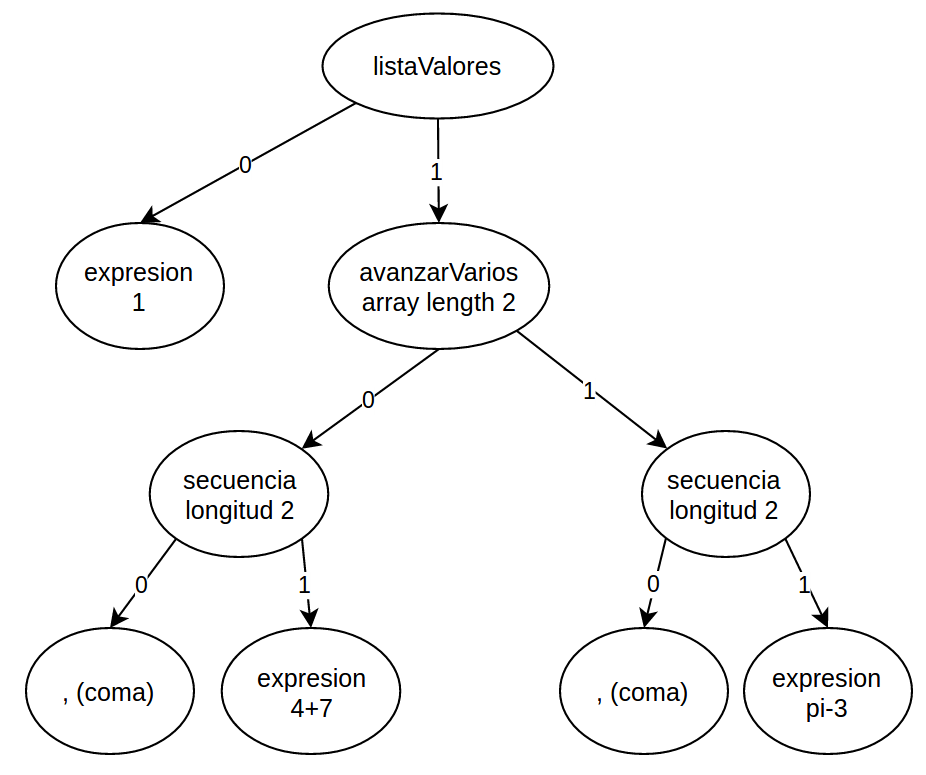
\includegraphics[width=0.5\linewidth]{analisisejemplo}
	\caption[Ejemplo de análisis.]{En este diagrama, this.resultado(1) es el nodo avanzarVarios. this.resultado(1)[i] es la i-ésima secuencia compuesta de una coma seguida de una expresión. this.resultado(1)[i][1] es la expresión de tal secuencia.}
	\label{fig:analisisejemplo}
\end{figure}


	Después se puede ver como se define un array, al que se le van a concatenar los `expresion' ignorando la coma (que es un separador y no tiene interés semántico). Para entender bien la línea this.resultado(1)[i][1], en la \hyperref[fig:analisisejemplo]{figura 5.2} se puede ver el esquema del árbol de resultados generado al analizar 1,4+7,pi-3:

	\vspace{10px}

	Tomando como último ejemplo el si condicional, estructura algorítmica que puede llevar concatenado otro si condicional (equivalente a un else):
	
	
\begin{BVerbatim}
{
  // Romper la ambiguedad LL(3) entre
  // si no x hacer
  // si no hacer
  try {
    this.avanzar("si")
      .avanzar("no")
      .avanzar("hacer")
  } catch (e) {
    if (!zl.error.esError(e))
      throw e;
    // Si no se puede hacer el si no hacer, intentar la reducción de verdad
    this.retroceder(this.arbol().length);
    this.avanzar("si")
      .expresion()
      .avanzar("hacer")
      .acumular("sentencia").avanzarVarios();
    this.intentar([
      ["fin"],
      ["sinocondicional"],
      ["sino"]
    ]);
    var intento = this.resultado(4);
    if (intento == 0) {
      this.registrarResultado({
        condicion: this.resultado(1),
        sentencias: this.resultado(3)
      });
    } else {
      this.registrarResultado({
        condicion: this.resultado(1),
        sentencias: this.resultado(3),
        siguiente: this.resultado(4, intento, 0)
      });
    }
    return this;
  }
  // Si no se llama al catch, es porque se pudo hacer un si no hacer.
  // En el caso de si no hacer, retroceder 3 y lanzar error:
  this.retroceder(3);
  throw zl.error.newError(zl.error.E_SIMBOLO, this.arbol());
});
\end{BVerbatim}
	
	Esta regla es más compleja ya que contiene el código explícito que rompe una ambigüedad de tres tokens: `si no hacer'/`si no \{expresion\} hacer'. La primera equivale a un \textit{else} en C y la segunda a un \textit{if(!\{expresion\})} en C (negación de una expresión dentro de una condición). La lógica detrás del algoritmo para romper la ambigüedad es la siguiente: se intenta (con try) avanzar si-no-hacer. Si se consigue, entonces no es un \textbf{sicondicional} (es un \textbf{sino}), se retrocede 3 tokens y se lanza una excepción. Con esto se consigue que el algoritmo de análisis intente la siguiente opción posible, y descarte el \textbf{sicondicional}. 
	
	\vspace{10px}
	
	En caso de que el intento si-no-hacer falle (se capture una excepción), se descarta la ambigüedad y se intenta avanzar la regla sin problemas. Para distinguir si la excepción capturada es a causa de un error en el análisis o de un error de Javascript utilizo la función \textit{esError} de la biblioteca zl.error, que devuelve verdadero si el objeto capturado en la excepción es un error zl. En caso de que el error no sea de análisis lo propago.
	
	\vspace{10px}
	
	Por otro lado, en el fichero \textbf{entorno.js} se definen las distintas clases que componen la tabla de símbolos. Cada clase tiene un método rellenarDesdeArbol que recibe un árbol como el generado en las reglas para rellenar cada uno de los elementos de la tabla. Por ejemplo, si vemos el objeto que se rellena en la regla subrutina, y vemos el método rellenarDesdeArbol de subrutina \footnote{La subrutina no se incluye completa, solo la parte que genera el árbol.}:
	\begin{BVerbatim}
Subrutina.prototype.rellenarDesdeArbol = function(arbol) {
  // Posicion de la subrutina:
  this.posicionSubrutina = [arbol.begin, arbol.end];
  this.posicionCabecera = arbol.secciones.cabecera;
  this.posicionDatos = arbol.secciones.datos;
  this.posicionAlgoritmo = arbol.secciones.algoritmo;

  this.nombre = arbol.nombre.toLowerCase();

  // Registrar modificadores
  for (var i = 0; i < arbol.modificadores.length; i++) {
    this.modificadores[arbol.modificadores[i].toLowerCase()] = true;
  }

  // Registrar primitivas:
  if ("primitiva" in this.modificadores) {
    // Extraer del segmento el código:
    this.segmentoPrimitivo = 
      arbol.segmentoPrimitivo.substring(2, arbol.segmentoPrimitivo.length - 2);
  }

  // Registrar datos
  for (var i = 0; i < arbol.datos.length; i++) {
    var decl = new Declaracion(this);
    decl.rellenarDesdeArbol(arbol.datos[i], this.padre);

    if (decl.nombre in this.declaraciones)
      throw zl.error.newError(zl.error.E_NOMBRE_DATO_YA_USADO, {
        posicion: [arbol.datos[i].begin, arbol.datos[i].end],
        arbolDato: arbol.datos[i],
        otroDato: this.declaraciones[decl.nombre]
      });
    else
      this.declaraciones[decl.nombre] = decl;

    // Registrar si es global:
    if (decl.modificadores & decl.M_GLOBAL) {
      this.padre.registrarGlobal(decl);
    }
  }
...
}
	\end{BVerbatim}
	
	Se puede ver al principio como se usa la información que se registra en el árbol para preparar la estructura de la subrutina. Se copian el nombre, las secciones, se guarda una tabla de los distintos modificadores, en caso de subrutina primitiva se extrae el código... Pero quizá el punto más interesante sea el registro de los datos: por cada dato a registrar se pide una instancia nueva de Declaracion, que se rellena usando rellenarDesdeArbol y pasando la rama del árbol relativa a la declaración. También se comprueba que no haya dos datos con nombres repetidos, en cuyo caso se lanza una excepción. 
	
	\subsection{Análisis semántico}
	
	Parte del análisis semántico se hace en el apartado anterior. Mientras se genera la tabla de símbolos se comprueban la existencia de elementos duplicados (dos subrutinas o dos datos con el mismo nombre), además de modificadores ilegales (por ejemplo, un dato no puede ser global y de entrada al mismo tiempo). Sin embargo, después de generar la tabla de símbolos hay que hacer comprobaciones que no tienen que ver con los símbolos, sino con los algoritmos, las operaciones y sus tipos. Estas últimas comprobaciones antes de generar el código Javascript se encuentran en (\textbf{semantica.js}). 
	
	\vspace{10px}
	
	Para poder realizar estas comprobaciones hay que obtener el tipo de datos resultado de cada expresión. Para ello hace falta haber generado previamente la tabla de símbolos para conocer los tipos asociados a ciertos nombres, así como los operadores definidos para ciertos tipos\footnote{ZL permite la sobrecarga de operadores.}.
	
	\vspace{10px}
	
	Cuando se analiza una expresión en busca de su tipo puede que el tipo ya esté calculado (si el nodo del árbol de la expresión tiene el miembro \textit{tipofinal}). Si no está calculado, se usa la función \textbf{testarExpresion} en \textbf{semantica.js} que usa una aproximación \textit{divide y vencerás} para obtener el tipo de la expresión. Si la expresión es simple (está compuesta por solo un elemento, como un nombre o una constante) el tipo se obtiene de forma trivial (mirando en la tabla de símbolos si es un nombre, o mirando en el árbol si es una constante). Si la expresión está compuesta de un operador (binario o unario) y unos (o un) operando, se obtiene el tipo final de cada una de las partes, y se comprueba si existe operador para estos tipos de datos.

	\vspace{10px}
	
	El proceso de análisis semántico es un proceso recursivo que parte del árbol de análisis generado en el primer proceso. Desciende en el árbol por todas las subrutinas para hacer las siguientes comprobaciones semánticas en las sentencias, y emitiendo una excepción\footnote{La lista de errores que se emiten como excepción se puede encontrar en error.js} en caso de no cumplirse:
	
	\vspace{10px}
	\noindent
	\textbf{La estructura bucle mientras, así como los condicionales tienen que tener una expresión cuyo tipo sea booleano}. Esta comprobación es la misma que se puede encontrar en Java por ejemplo. La expresión se evalúa a verdadero o falso para ver si hay que saltar o no (en el caso condicional) o para ver si hay que continuar o no (en el caso bucle mientras).
	
	\vspace{10px}
	\noindent
	\textbf{La estructura bucle repetir tiene que tener una expresión cuyo tipo sea número}. De la expresión numérica se obtiene la parte entera, y de ahí el número de veces que se va a repetir el bucle, por eso tiene que ser de tipo número. 
	
	\vspace{10px}
	\noindent
	\textbf{La expresión en una asignación, o en un argumento de entrada en una llamada tiene que ser del mismo tipo}. Si una asignación no coincide en tipo podría haber problemas no deseados en tiempo de ejecución. Aquí sucede como en Java o C++, salvo que en ZL no hay conversiones explícitas.
	
	\vspace{10px}
	\noindent
	\textbf{No existe la operación para un operador y unos tipos operandos dados}. Para poder conocer el tipo de datos del resultado de cada expresión deben existir operadores compatibles. Esta exigencia se cumple en otros muchos lenguajes también, como Java o C++. Por ejemplo, si el operador suma binaria (· + ·) no está definido para dos booleanos la expresión `verdadero + falso' no pasaría esta comprobación.
		
		
	%TOOD: Cita al type casting.
	\vspace{10px}
	\noindent
	\textbf{Para poder usar la operación de conversión de tipos debe existir una subrutina conversora}. En C o C++ existe una fórmula similar que se llama \textit{type casting}. En ZL para convertir un valor de un tipo A en un valor de un tipo B se puede definir una subrutina con el modificador conversora que reciba el valor tipo A y emita un valor tipo B equivalente, pero para usar el conversor de forma semánticamente correcta debe existir tal conversor. 
		
	\vspace{10px}

	\subsection{Código nativo, implementación de las subrutinas ZL nativas}
	
	%TODO: cambiar esta sección por generación de código
	
	El nombre de código nativo suele referirse en el contexto informático como el código que es capaz de ejecutar directamente una CPU. En el contexto de este trabajo, me refiero a código nativo como código no para la CPU (en ensamblador) sino como código en Javascript, que puede ser evaluado por la plataforma web. 
	
	\vspace{10px}
	
	Las subrutinas de código ZL se transforman a funciones de Javascript, pudiendo estas evaluarse y llamarse. Se puede decir que hay un mapeo de todas las subrutinas a funciones. Sin embargo, esto no es suficiente para producir un entorno de ejecución útil. Si las subrutinas de ZL solo pudieran llamar a otras subrutinas ZL, y ninguna de ellas fuese provista de código nativo, obtendríamos un entorno sin entradas ni salidas. 
	
	\vspace{10px}
	
	Para poder dotar de utilidad al sistema hay que incluir al entorno de ejecución subrutinas que, usando código nativo, permitan las operaciones de entrada y salida. En ZL existen dos formas de insertar en el entorno de ejecución subrutinas con código nativo: definir una función Javascript y vincularla a una clase Subrutina, añadiéndola artificialmente a la tabla de símbolos, o escribir dentro de un código ZL código Javascript embebido de alguna forma (como se hace con JSNI para GWT \cite{jnsigwt}). Se sugiere siempre que sea posible se use la segunda forma, ya que alterar la tabla de símbolos es más complejo.
	
	\vspace{10px}
	
	Parte del código nativo de ZL está en \textbf{ejecucion.js}, que contiene los tipos de datos nativos. La otra parte en \textbf{bibliotecasZL/*.zl} contiene las funcionalidades del lenguaje. Dentro de la carpeta \textbf{bibliotecasZL} hay repartidos ficheros de código fuente escritos en ZL con código Javascript embebido.
	
	\vspace{10px}
	
	\label{subrutinasprimitivas}
	El mecanismo más sencillo para implementar código nativo Javascript en ZL es el segundo mecanismo; usar una subrutina primitiva. Cuando una Subrutina escrita en ZL lleva el modificador `primitiva' entonces en vez de algoritmo recibe un comentario multilínea con código en Javascript, que se copia tal cual a la hora de compilar a Javascript (ver \hyperref[fig:zlyjs]{figura 5.3}).
	
	\vspace{10px}
	
	Como se puede ver en la imagen, se usa \textbf{\textit{\$entrada.x}} para acceder al dato de entrada con nombre x. Como el lenguaje es insensible, los nombres se serializan todos en minúscula. Además de la variable \$entrada, existen también las variables \textbf{\$salida} (para escribir datos de salida), \textbf{\$miembros} (para escribir datos globales), \textbf{\$local} (para datos locales, aunque en Javascript se puede usar directamente la palabra `var'), y \textbf{\$exterior} para acceder a recursos exteriores (como el lienzo para dibujar, por ejemplo). 
	
\begin{figure}
\centering
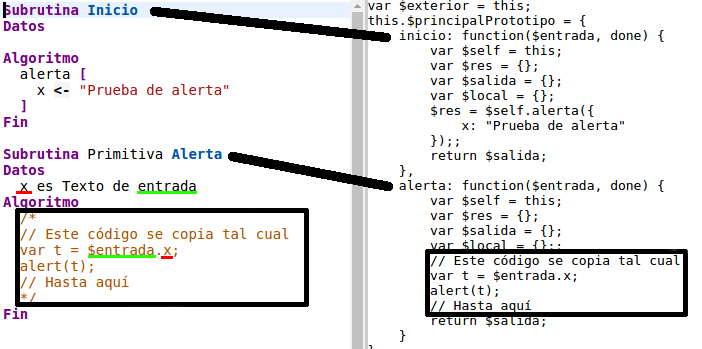
\includegraphics[width=1\linewidth]{zlyjs}
\caption[Ejemplo de código generado y código nativo.]{La subrutina inicio se compila de ZL a JS. Sin embargo, la subrutina Alerta solo se añade a la tabla de símbolos y se copia tal cual.}
\label{fig:zlyjs}
\end{figure}
	
	Con ese código nativo sencillo se da pie a poder usar la utilidad \textbf{alert} del explorador, como se puede ver en la \hyperref[fig:alert]{figura 5.4}.
	
\begin{figure}
\centering
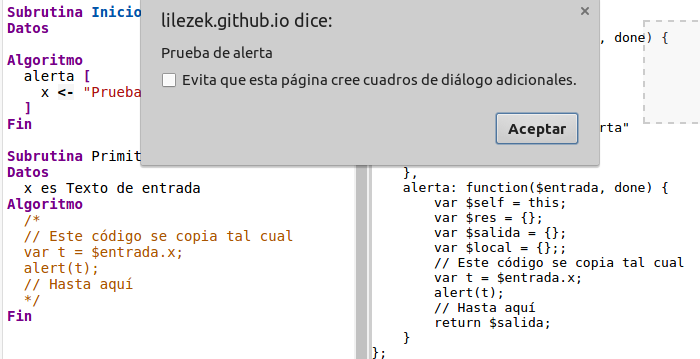
\includegraphics[width=1\linewidth]{alert}
\caption[Código nativo que muestra una alerta.]{El código embebido en Javascript permite el uso de la funcionalidad \textit{alert}, que recibe un literal desde ZL y lo muestra correctamente.}
\label{fig:alert}
\end{figure}

	\vspace{10px}
	
	
	
	\vspace{10px}
	
	Se recomienda al lector que si quiere avanzar en el proceso de escritura de código nativo para comunicarse con el `exterior' que mire los códigos en \textbf{bibliotecasZL/*.zl}, especialmente \textbf{basico.zl}.
	
	\subsection{Código asíncrono convertido a código bloqueante}
	
	Javascript usa el paradigma de código asíncrono \cite{javascriptasync}. `Romper' ese paradigma para que ZL corra de forma bloqueante sobre Javascript ha sido, sin duda alguna, la parte más compleja de todo el proyecto. 
	
	\vspace{10px}

	Allá donde una función en Javascript pueda bloquear la ejecución para hacer una acción de entrada/salida siempre habrá que usar llamadas asíncronas. Las llamadas asíncronas se caracterizan por ceder la CPU inmediatamente a la siguiente línea de código, y a llamar a otra función llamada `callback' cuando la acción de entrada/salida haya terminado. El siguiente ejemplo:
	
\begin{BVerbatim}
xhttp.open("GET", "imagen.png", false);
xhttp.send();

// Usar imagen aquí

\end{BVerbatim}

	Obtiene una imagen de forma síncrona. Si el servidor que la hospeda tarda 4 segundos en responder, el explorador web se quedará congelado 4 segundos, cosa que no es aceptable. Además, existen otros escenarios donde el explorador se quedaría congelado una cantidad arbitraria de tiempo (por ejemplo, cuando el IDE le pide al usuario escribir un valor y hay que esperarlo).
	
	Para usar correctamente las utilidades asíncronas hay que usar un callback:


\begin{BVerbatim}
xhttp.onreadystatechange = function callback() {
 if (xhttp.readyState == 4 && xhttp.status == 200) {
  // Usar imagen aquí
 }
};
xhttp.open("GET", "imagen.png", true);
xhttp.send();
\end{BVerbatim}

	\vspace{10px}

	El problema de usar `callbacks' se puede resumir básicamente en que el orden en el que se ejecuta el código deja de ser lineal y de arriba a abajo. Un problema común en Javascript es el \textit{callback hell}\cite{callbackhell}, que hace que el código se ejecute dando saltos de forma inevitable. 
	
	Para avanzar en materia, se definen los siguientes puntos:
	
	\noindent
	Un \textbf{callback} es una función que indica el punto de salida de una función asíncrona. Si bien una función clásica en C o en Javascript empieza en la primera línea de código y acaba en un \textit{return} (o al final si no hay \textit{return} alguno), en una función asíncrona el final lo representa el callback.  
	
	\vspace{10px}
	
	\noindent
	\textbf{El cometido de una función asíncrona no acaba con un return. Acaba cuando se llama al `callback'.} Por lo general, cualquier función asíncrona hace return antes de llamar al callback, rompiendo el orden.
	
	\vspace{10px}
	
	\noindent
	\textbf{Toda función A que contenga una llamada asíncrona B es asíncrona.} Ya que no se puede bloquear la ejecución de B en Javascript, la llamada asíncrona B solo acaba cuando se llame al callback, y A debe preparar un callback también.
	
	\vspace{10px}
	
	\noindent
	\textbf{Si entre una secuencia de código A y otra B, se introduce una llamada asíncrona, la secuencia de código B se ejecutará antes de que la llamada asíncrona finalice.} Por lo tanto, si se quiere mantener el orden, hay que mover el código B dentro de un callback, y ofrecer ese callback a la llamada asíncrona.
	
	\vspace{10px}
	\noindent
	\textbf{Si un \textit{if} condicional contiene una llamada asíncrona, todo el \textit{if} condicional se vuelve asíncrono pero no necesariamente los \textit{elseif}-\textit{else}}. Esto se debe a que si la condición del \textit{if} no se cumple, no se hace la llamada asíncrona. Sin embargo, la estructura que contenga el \textit{if} condicional sí será asíncrono. 
	
	\vspace{10px}
	\noindent
	\textbf{Si un bucle (repetir, o mientras) contiene una llamada asíncrona, el bucle completo se vuelve asíncrono}. Además, hay que romper cada iteración del bucle para llamar a la siguiente iteración solo después de que acabe el callback de la última llamada asíncrona.
	
	\vspace{10px}
	\noindent
	\textbf{Si una estructura (función, bucle, sí condicional) contiene otra estructura asíncrona, la estructura se vuelve a su vez asíncrona}. Esto es equivalente al segundo punto, una función asíncrona convierte en asíncronas a todas las funciones que la llaman.
	
\begin{figure}
	\centering
	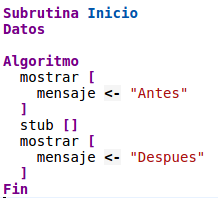
\includegraphics{asincrono}	
	\\
	
	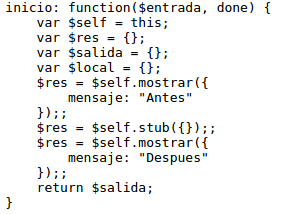
\includegraphics[width=0.45\linewidth]{asincrono3}
	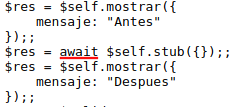
\includegraphics[width=0.45\linewidth]{asincrono2}

	\caption[Diferencias entre código asíncrono y síncrono.]{Arriba, código ZL de ejemplo. A izquierda, código Javascript autogenerado donde stub es una llamada síncrona. El código de ZL se ejecuta en el mismo orden que el código en Javascript. A la derecha, stub pasa a ser una llamada asíncrona. Hay que romper el código en varias fases para poder pasar los callbacks. En la imagen de la derecha, en rojo se ven los bloques de antes y después de la llamada asíncrona, y entre ambos la llamada a stub. En verde, las llamadas a los callbacks.}
\label{fig:asincrono}
\end{figure}


	 Ejemplificando, se puede ver en la \hyperref[fig:asincrono]{figura 5.5} como se utiliza \textit{async.waterfall}, una utilidad\cite{async} que simplifica la ejecución en cascada de trozos asíncronos.
	 
	 \vspace{10px}
	 
	 La función async.waterfall recibe un array de funciones, que se comportan de una forma específica: todas ellas van a recibir como último argumento una función, a la que se le va a llamar \textit{done}. Después del array recibe una última función, a la que llamamos \textit{callback}.
	 
	 \vspace{10px}
	 
	 Cuando una función acabe su cometido asíncrono, debe llamar a su último argumento: a la función \textit{done}. Al llamar a esa función se le da paso a la siguiente función. A la función \textit{done} se le debe llamar con el primer argumento nulo, y el resto de argumentos se pasarán a la siguiente función. El primer argumento se usa para propagar un error, pero si es nulo no se propaga nada.   
	 
	 \vspace{10px}
	 
	 Salvo la primera función que solo recibe la función \textit{done}, el resto de las funciones reciben como argumentos los argumentos pasados en la función anterior a través de \textit{done}. La última función, al llamar a \textit{done}, en vez de dar paso a la siguiente función (pues no existe) lo que sucede es que se llama a la función `callback'.
	
	\section{Editor inteligente}
	
	Cuando se habla de editor inteligente se puede entender el funcionamiento del editor a ayudar a escribir el código y a simplificar su lectura, coloreando el texto, sugiriendo nombres, etc... Por ejemplo, si se usase un editor inteligente para Java, se esperaría ayuda con los nombres, ya que por ejemplo la clase JButton tiene más de 350 métodos. Acordarse de todos es una tarea compleja, y por eso los editores modernos tienen sistemas de autocompletado. 
	
	\vspace{10px}
	
	\subsection{Autocompletado}
	
	Por autocompletado se puede entender toda forma de generar código automáticamente. Tal código generado debe ser útil para el que lo escribe, y para ello el editor se puede adelantar a lo que escribe el usuario. En la práctica el autocompletado se puede ver para reducir el código a escribir (el editor completa el resto), y recordar nombres y estructuras (que el editor puede conocer mediante análisis del contexto).
	
	\vspace{10px}
	
	El IDE de ZL tiene coloreado de sintaxis (definido en \textbf{editor.js} y \textbf{editor.css}), un cursor más grueso de lo habitual y coloreado de líneas (de error, de escritura y de pausa). Además del coloreado, el IDE tiene un sistema de autocompletado con análisis del contexto.
	
	\vspace{10px}
	
	El IDE está configurado para compilar el código después de un cierto tiempo (0.25 segundos) si el usuario no teclea. Con ello se consigue ocultar al usuario la \textbf{fase de compilación}, volviéndola \textbf{automática}. 
	
	\vspace{10px}
	
	El sistema de autocompletado parte de un \textit{addon} de CodeMirror que se configura en el fichero \textbf{autocompletado.js} y que tiene toda la lógica de autocompletado. Dentro del fichero se encuentran los algoritmos que determinan el contexto, filtran las posibles sugerencias y las ordena por unos criterios de (posible) importancia para el programador.
	
	\subsection{Determinando el contexto}
	
	Determinar el contexto de la escritura en el editor se puede separar en dos fases: estudiar el contexto según la posición del ratón para ofrecer sugerencias, y estudiar el conjunto de nombres y tipos para autocompletar correctamente las llamadas.
	
	\vspace{10px}
	
	El contexto se determina siempre en base a la última tabla de símbolos generada. Es decir, la última compilación no fallida se almacena para el uso del autocompletado. La primera fase para determinar el contexto es ver `donde' está localizado el cursor. Se puede saber si el cursor está dentro de una subrutina o fuera ya que las subrutinas guardan en sus estructuras la posición de inicio y final de cada una de sus partes. 
	
	\vspace{10px}
	
	Si el cursor está fuera de una subrutina lo único que tiene cabida es escribir una subrutina. Por eso, si se fuerza el autocompletado (Ctrl-Espacio o Cmd-Espacio) se obtiene una nueva subrutina de nombre `Nombre'.
	
	\vspace{10px}
	
	Si el cursor está dentro de una subrutina el autocompletado se vuelve más complejo. En la sección de datos se deben sugerir las palabras clave global, entrada, salida, así como los tipos de datos ya registrados. Por otro lado, si el cursor está dentro de la sección algoritmo, las sugerencias se vuelven más complejas todavía. Hay que sugerir las distintas estructuras algorítmicas así como las distintas llamadas y nombres de datos (\hyperref[fig:autocompletado]{figura 5.6}).
	
\begin{figure}
\centering
	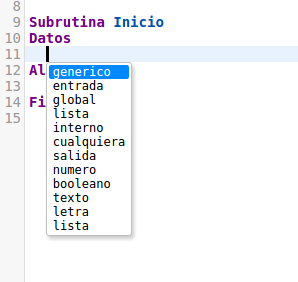
\includegraphics[width=0.45\linewidth]{autocompletado2}
	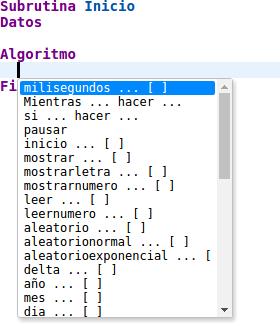
\includegraphics[width=0.35\linewidth]{autocompletado3}
\caption[Ejemplos de distintos contextos en autocompletado.]{A izquierda, el contexto para declarar nuevos datos. A la derecha, las opciones relacionadas con los algoritmos.}
\label{fig:autocompletado}
\end{figure}
	
	\vspace{10px}
	
	Lo último destacable de los algoritmos de contexto es que para no perder el correcto funcionamiento, cada vez que se inserta o se borra un carácter, se `mueven' todos los índices de subrutinas. Por ejemplo, si una subrutina empieza en 14 y acaba en 67, si se eliminan dos caracteres dentro de la subrutina se mueven los índices (de todas las subrutinas) y en concreto esa subrutina empezaría en 14 y acabaría en 65.
			
	\subsection{Algoritmos de similitud de nombres}
	
	Para poder sugerir correctamente es importante ordenar las posibles sugerencias de mayor a menor `utilidad'. La utilidad se podría medir como la capacidad del editor a sugerir una opción A por encima de la opción B, siendo la opción A la que el programador realmente busca. Para ello el entorno de programación implementa algoritmos heurísticos (no aprenden sobre la marcha) que determinan el grado de utilidad según lo similar que son el texto que está actualmente escribiendo el programador y los nombres de las sugerencias (este método lo usan editores como Eclipse y Visual Studio).
	
	\vspace{10px}
	
	En un principio planteé el uso del algoritmo `subsecuencia común más larga'\cite{lcs}, que localiza la subsecuencia (subconjunto de caracteres en un texto respetando el orden) más larga entre un texto y otro. Esta es la solución que usa la utilidad `diff'\cite{diff} para evaluar las diferencias. Sin embargo, después varias pruebas, opté por usar otro algoritmo: el algoritmo de distancias de edición\cite{levensthein}, que penaliza en menor medida los textos desordenados.
	
	\vspace{10px}
	
	Las diferencias notables entre un algoritmo u otro son:
	
	\vspace{10px}
	
	\noindent
	\textbf{LCS}: penaliza los desórdenes. Por definición, una subsecuencia siempre respeta el orden. Escribir imilsegundo da casi la misma puntuación a milisegundo que a segundo. Sin embargo, Levensthein acepta el desorden como parte del algoritmo y puntúa mejor en ese caso.
	
	\vspace{10px}
	\noindent
	\textbf{Levensthein}: penaliza la diferencia de tamaños. Como Levensthein es una distancia, la suma +1 a las inserciones hace que `raton' puntúe mejor `redondearbajo' que `esconderaton'. En este mismo caso LCS puntuaría mejor `esconderaton' por poder encajar las 5 letras de ratón en una subsecuencia.
	
	\vspace{10px}
	
	A demás de sugerir en el autocompletado, los algoritmos de similitud de nombres se usan también para autocompletar las llamadas, siempre que el contexto sea correcto. Las dos siguientes llamadas están autocompletadas (\hyperref[fig:autocompletado2]{figura 5.7})
	
\begin{figure}
\centering
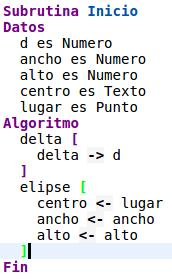
\includegraphics[width=0.4\linewidth]{autocompletado}
\caption[Autocompletado con filtro por tipos]{Las asignaciones de los argumentos en las llamadas se hace por similitud de nombres, además de por contexto. La elipse recibe como centro un tipo punto y por eso se escoge lugar antes que centro, aunque no coincidan en nombre.}
\label{fig:autocompletado2}
\end{figure}

	
	\subsection{Errores y pausas}
	
	El entorno ofrece un mecanismo para mostrar los errores que se comenten al escribir código. Se colorea en rojo la línea en la que se encuentra el error. Los generadores de la información por error se puede encontrar en \textbf{error.js} (y el estilo en \textbf{error.css}). Existe una clase Error que se usa para distinguir de cualquier Excepción del lenguaje que no sea un error ZL (por si se comete un error escribiendo el código Javascript del IDE).
	
	\vspace{10px}
	
	Cada vez que en una fase de análisis se localiza un error (sintático o semántico) se escoge un constructor de error (dependiendo del error cometido se escoge un constructor u otro). Al constructor se le pasa el árbol sintáctico generado así como información adicional donde sea necesario (por ejemplo, si se definen dos veces la misma subrutina, se pueden pasar el trozo del árbol de ambas subrutinas). Un ejemplo de constructor de error puede ser el siguiente (cuando se llama a una subrutina con datos incompatibles):
	
	\begin{BVerbatim}
zl.error.E_LLAMADA_DATO_INCOMPATIBLE = function(informacion) {
 // Identificadores únicos
 this.enumeracion = 10; 
 this.identificador = "E_LLAMADA_DATO_INCOMPATIBLE"; 
 // Información del error
 this
  // Resalta en rojo la línea de error y genera un indicador
  .resaltarLinea(informacion.posicion[0]) 
  .texto("En la llamada a ")
  .subrutina(informacion.dato.padre)
  .texto(" el dato ")
  .dato(informacion.dato)
  .nuevaLinea()
  .texto(" debería ser de tipo ")
  .tipo(informacion.esperado)
  .nuevaLinea()
  .texto(" pero el valor dado es de tipo ")
  .tipo(informacion.obtenido)
}
	\end{BVerbatim}
	
	\begin{figure}
		\centering
		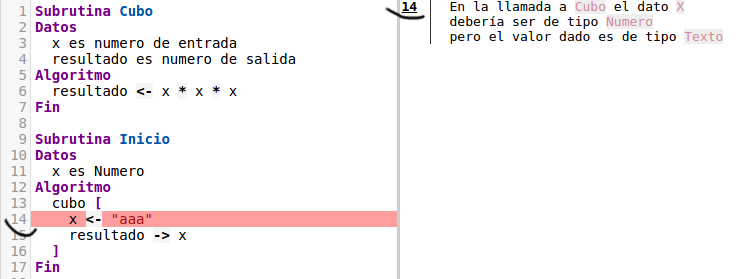
\includegraphics[width=1\linewidth]{error}
		\caption[Ejemplo de código erróneo y mensaje de error.]{A la izquierda el código erróneo (cubo es una subrutina que eleva al cubo el valor x), y a la derecha el mensaje de error mostrado por el código erróneo.}
		\label{fig:error}
	\end{figure}
	
	Si se comete un error programando (ver la \hyperref[fig:error]{figura 5.8}), se genera un código HTML como el siguiente:
	
	\vspace{10px}
	
	\begin{BVerbatim}
<div class="error">
<span class="linea" onclick="saltarAlCodigo(14,0);">14</span>
En la llamada a <span class="subrutina">cubo</span> el dato 
<span class="dato">x</span>
<br> debería ser de tipo <span class="tipo">numero</span>
<br> pero el valor dado es de tipo <span class="tipo">texto</span>
</div>
	\end{BVerbatim}
	
	\vspace{10px}
	
	Además de la representación gráfica de errores, el IDE tiene construido un sistema para poder detener la ejecución del código. Como se ha visto en la sección  `Código asíncrono convertido en código bloqueante', existe un mecanismo para bloquear la ejecución de código Javascript que espera a un evento y después llama a un `callback' para continuar. Aprovechando este mismo mecanismo, se puede pausar la ejecución del código como si hablásemos de \textit{breakpoints}\cite{breakpoint}, esperando al evento de que el usuario pulse `continuar' (ver \hyperref[fig:pausa1]{figura 5.9}).
	
	
	
\begin{figure}
\centering
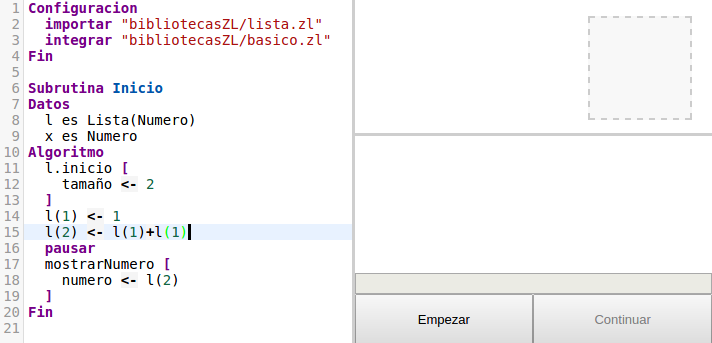
\includegraphics[width=0.45\linewidth]{pausa1}
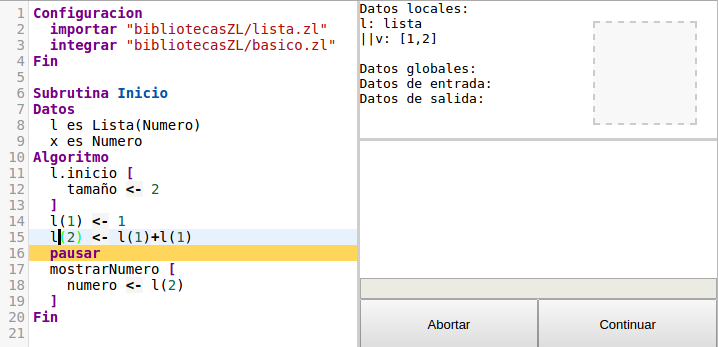
\includegraphics[width=0.45\linewidth]{pausa2}
\caption[Ejemplo de uso de pausa (breakpoint).]{A izquierda, el IDE antes de `Empezar' la ejecución. A la derecha, el IDE tras pasar por la sentencia `pausar'. Durante la pausa se muestra información de depuración, pero hay que activarlo pulsando Ctrl+F9 (Cmd+F9 en Mac OS X en teoría, no se ha podido probar por falta de material).}
\label{fig:pausa1}
\end{figure}
	
	\section{Triple plataforma - Web, Electron y NodeJS}
	
	%TODO: Eliminar para ahorrar espacio
	
	Este trabajo principalmente funciona sobre Web, pero se ha programado para ser compatible con tres plataformas distintas. 
	
	Además del IDE web existen otras dos plataformas (menos probadas y que podrían contener errores) basadas en NodeJS (ejecución de scripts Javascript de forma independiente) y Electron (un entorno similar al web pero sin necesidad de un explorador). NodeJS permite la ejecución de código sin IDE, que puede ser útil para implementar por ejemplo un juez online como el que tiene iJava en el proyecto Descubre. NodeJS ejecuta código Javascript fuera del explorador, al igual que se ejecutaría Python o Perl. 
	
	\vspace{10px}
	
	Además, en el proyecto actualmente se usa NodeJS para hacer pruebas unitarias. Se puede usar NodeJS para compilar unos ejemplos y comprobar que siguen compilando en un futuro. 
	
	\vspace{10px}
	
	Por otra parte Electron permite tener multiples ventanas para, por ejemplo, separar el lienzo de dibujado del editor de código, haciendo que la interfaz de usuario del entorno pueda ser más flexible. 
	
	\chapter{Conclusiones y vías futuras}
	
	Este trabajo ha tenido como objetivo crear un entorno sin instalación que permita convertir un lenguaje cercano al lenguaje natural en instrucciones, para que alumnos sin conocimientos puedan iniciarse en la programación. 
	
	Las metas propuestas se han logrado ya que se ha conseguido un compilador para el lenguaje, que está en castellano y es sencillo de leer, así como el entorno que une el editor y el compilador en uno. 
	
	El entorno con el lenguaje ofrece funcionalidades similares a las que se pueden encontrar en el trabajo Descubre, que antes de que se plantease el proyecto fue el punto de inspiración. Con ZL se puede dibujar en un lienzo con llamadas imperativas así como escribir programas de entrada y salida de texto. 
	
	A todas esas funcionalidades se han añadido otras que parecían útiles como la capacidad de parar el código en un línea concreta. Poder parar la ejecución puede facilitar la comprensión del flujo de ejecución del código, que es una parte fundamental del pensamiento algorí 
	
	Para que el proyecto se pueda mejorar y se pueda continuar se ha puesto especial esfuerzo en que se pueda añadir funcionalidades al proyecto en forma de código nativo embebido en el código ZL. Así cualquier docente que encuentre útil esta herramienta podrá usarla para sus propios propósitos. 
	
	Otra posible forma de mejorar este trabajo sería someterlo a pruebas con distintos usuarios para comprobar el grado de utilidad. Las decisiones de diseño se han tomado en base a la experiencia personal, y podrían ser sometidas a encuestas para cambiar entre otras cosas las estructuras sintácticas o el léxico. 
	 
	
	 
	\bibliographystyle{amsplain}
	\bibliography{biblio}

	\appendix
	\chapter{Notación BNF (extendida) del lenguaje} \label{app:a}
	
	\VerbatimInput{../sintaxis.txt}
	
	\chapter{CodeCombat, imagen de la aplicación} \label{app:b}
	
	\begin{center}
	
\includegraphics[width=1\linewidth]{codecombat}
	
	A derecha, un editor de texto con el lenguaje de programación seleccionado. A izquierda, arriba, un lienzo con la situación del puzzle a resolver, y abajo un menú con información adicional (en esta imagen está en blanco tal menú).
	\end{center}
	
	\chapter{Ejemplo de expresión regular negative lookahead} \label{app:c}
	
	\begin{center}
		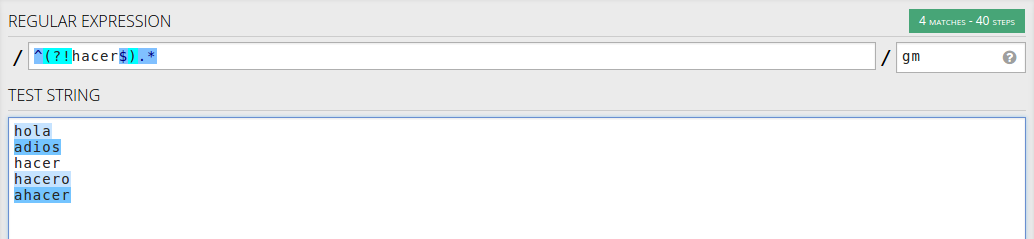
\includegraphics[width=1\linewidth]{negativelookahead}
		
		Arriba, la expresión regular con los modificadores global y multilinea.
		Abajo, el texto al que se le pasa la expresión regular. Como se puede ver, todo hace match salvo la palabra `hacer'.
	\end{center}
	
	\chapter{Khan Academy, ejemplo de error al programar} \label{app:d}
	
	\begin{center}
	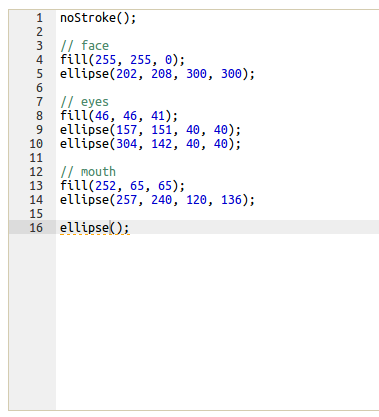
\includegraphics[width=0.45\linewidth]{khanerror}
	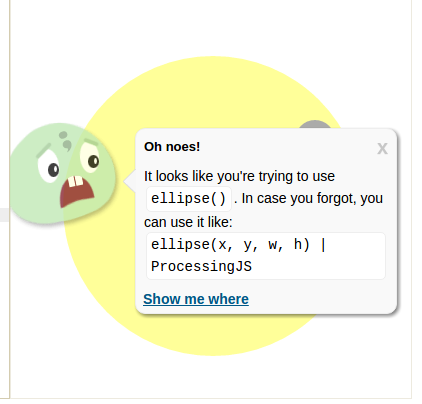
\includegraphics[width=0.45\linewidth]{khanerror2}
	
	A izquierda, cometo el error de escribir \textit{ellipse} sin argumentos, y a la derecha se puede ver como se usa un lenguaje poco formal (Oh noes! vs Error: signature of function...), acerca del error que he cometido.
	\end{center}
	

\end{document}